\chapter{Wing-box model} \label{chap:Model}
  
  %Intro
  A model of the whole wing-box including the variable-stiffness spar is developed to study the buckling characteristics of the chiral lattice, the response in twist of wing-box and the tailorability possibilities of that response. In the present chapter the model is presented, which in fact consists in two models one analytical and another one computational. 

  On first place, the working principle that lays under the proposed technology is presented. Next, the two different models developed to provide fully understanding of the structure response are presented. Firstly, a simple analytical model of a beam with a web featuring variable stiffness properties is presented. This is used to provide fast insight of the role of each of the design parameters on the final mechanical properties of the beam. Important relevance is given to the section's shear centre $y_{\mathrm{SC}}$ shifting. This variable determines the magnitude of the resulting torsional moment that acts on the beam as a result of a load applied on the beam's transversal plane, and that induces the beam twist.

  Secondly, the computational model is introduced. The different constituting elements are explained together with the boundary conditions, loads and mesh that are used in the simulations 

  Finally, the program used to carry out automatic parametric studies is presented, together with its methodology.

\section{Concept} \label{sec:concept_Model}
  %
  % Explanation of the concept
  % -> Bending-twist coupling
  % -> Shiftable shear centre location
  % -> A web with variable-stiffness capability
  %
  % Figure: Fig. 1 Raither ?, Geometry and system of coordinates.
  % Figure: Fig. 2 Raither ?, Schematic of the working principle.
  %
  %Chiral structure
  %View Airoldi (2012)
  %
  % -> Buckling phenomena
  % Figure: Schematic representation buckling phenomena

  As it was already introduced in last chapter, the proposed technology to achieve twist morphing through a variable torsional stiffness wing-box is based on the working principle presented in \cite{Raither2013a} and exploits the buckling characteristics of a lattice of chiral ligaments as a way of varying the effective shear modulus $G_{\mathrm{eff}}$ of the adaptive spar of the wing-box.

  The basic working principle can be understood considering a closed profile adaptive beam in which the shear centre is shifted as a result of the variable-stiffness capability of one of the webs. An schematic view of the working principle is shown in Figure \ref{fig:adaptive-beam-concept} where an adaptive beam is displayed. In Figure \ref{fig:adaptive-beam-concept}(a), the four webs that constitute the rectangular profile of the beam have the same shear stiffness $G_1 t_1 = G_2 t_2$. The double symmetry characteristic of such a configuration indicates that the shear centre is located at the point where the two symmetry axes intersect. For this case, under a load applied on the shear centre, the beam experiences bending deformation with zero twist. On the other hand, when considering the situation shown in Figure \ref{fig:adaptive-beam-concept}(b) where $G_1 t_1 > G_2 t_2$, the reduced shear stiffness of the adaptive web produces that shear centre moves along the $y$ direction and towards positive values of $y$. In this case, if the load is maintained in the same application point as before, the beam experiences bending deformation and negative twist. Correspondingly, for the case shown in Figure \ref{fig:adaptive-beam-concept}(c) where $G_1 t_1 < G_2 t_2$, the shifting of the shear centre is towards negative values of $y$ and the beam experiences a positive twisting under the prescribed load.

  \begin{figure}[!htpb]
    \centering
    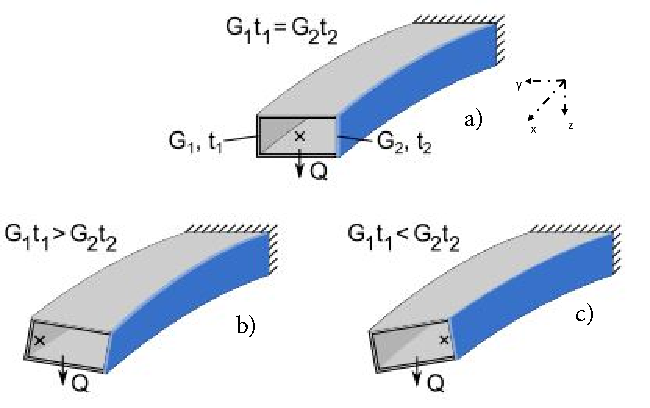
\includegraphics[width=0.7 \textwidth]{state-of-the-art/adaptive-beam-concept}
    \caption[Working principle for the adaptive beam]{Working principle for the adaptive beam. \cite{Raither2013}}\label{fig:adaptive-beam-concept}
  \end{figure}

  The bending-twist coupling of the beam can therefore be controlled by the variable-stiffness web. The properties of the web can be modified by either adjusting the shear modulus $G_2$ or the thickness $t_2$ of the adaptive web. 

  In the technology presented in this work, the adaptive web is constituted of a lattice of chiral structures. On these elements, elastic buckling is intentionally induced and the resulting consequence is the reduction of the overall shear modulus $G_2$ effectively introducing an effective shear modulus $G_{2,\mathrm{eff}} < G_1$. An example of the chiral structure undergoing buckling instabilities on some of the ligaments located at the wing-box root can be seen in Figure \ref{fig:exampleBuckling}.

  \begin{figure}[!htpb]
    \centering
    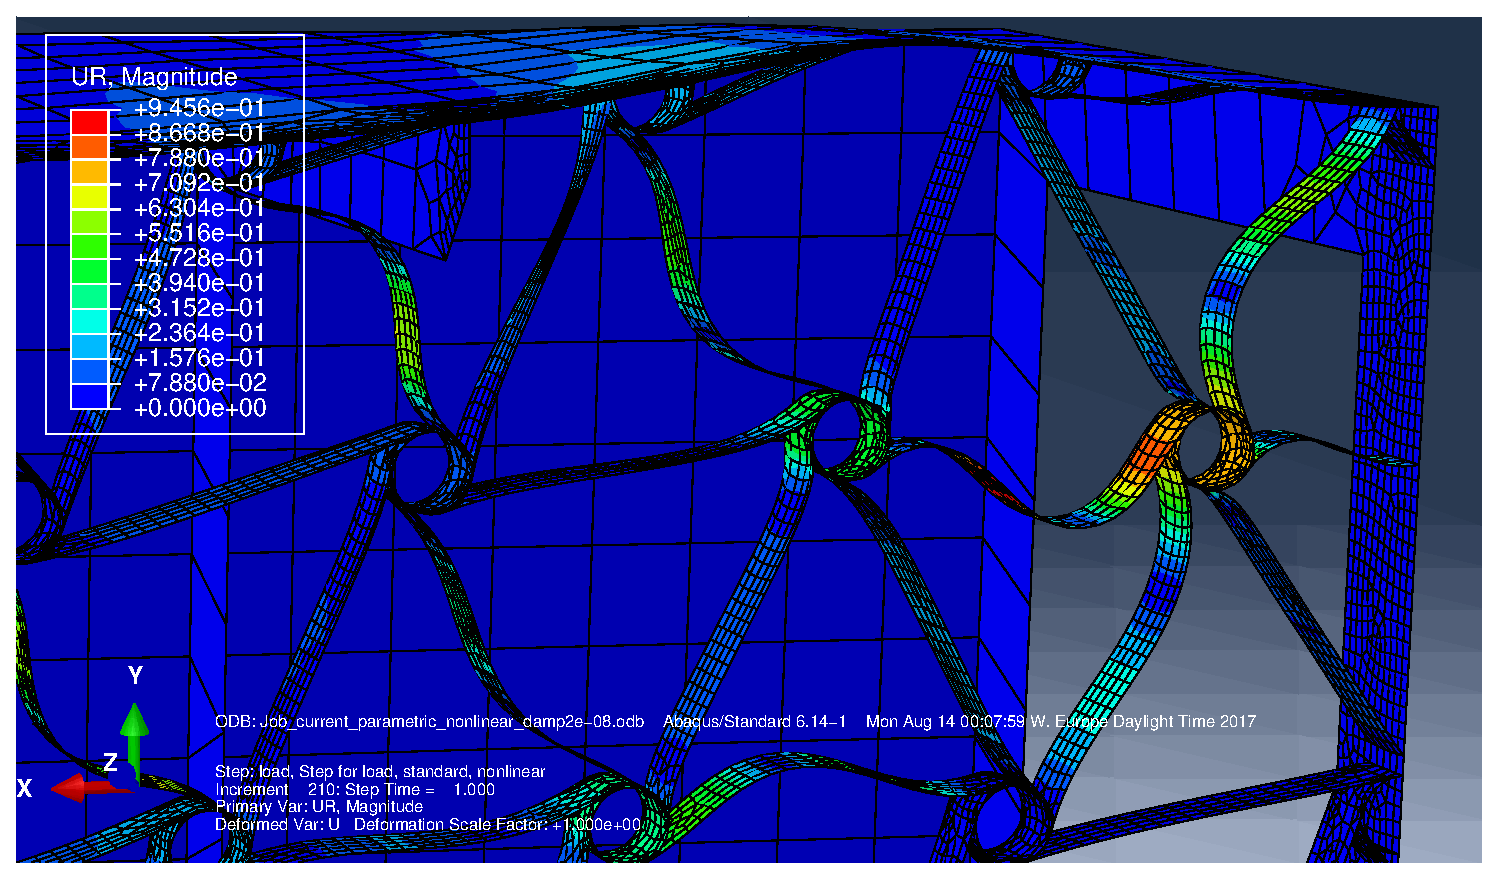
\includegraphics[width=0.7 \textwidth]{model/exampleBuckling}
    \caption[Set of chiral ligaments undergoing elastic instabilities at the root of the wing-box]{Set of chiral ligaments undergoing elastic instabilities at the root of the wing-box.}\label{fig:exampleBuckling}
  \end{figure}

  % wHAT'S THE ROLE OF ALL THIS IF BUCKLING IS NOW USED????
  % As shown in Section \ref{sec:chiral_state}, the negative Poisson’s ratio behavior leads to unique deformation patterns, and corresponds to a very high in-plane shear modulus $G$, as shown in Equation \ref{eq:shearModulus} for values of Poisson's ratio $\nu \to -1$:
  % %
  % \begin{equation}\label{eq:shearModulus}
  %   G = \frac{E}{2 (1 - \nu)},
  % \end{equation}
  % %
  % where $E$ is the Young's modulus. 
  %
\section{Analytical model} \label{sec:analytical_Model}
  %
  %% Analytical apprach description
  % An analytical model of the Wing Box will be build.
  % Shear centre calculation
  % The twist of the beam will be calculated
  %
  %Figure of analytical model

  The analytical model of the wing-box is described in the present section. An schematic view of the section of the beam can be seen in Figure \ref{fig:analyticalBox}. The main dimensions for the section are given by the height $H$ and the width $B$. Such a structure is characterized by having three elements with identical thickness $t_1$, shear modulus $G_1$ and Young's modulus $E_1$. For the element on the right, the adaptive web, the same parameters are $t_2$, $G_2$ and $E_2$, respectively. 

  \begin{figure}[!htpb]
    \centering
    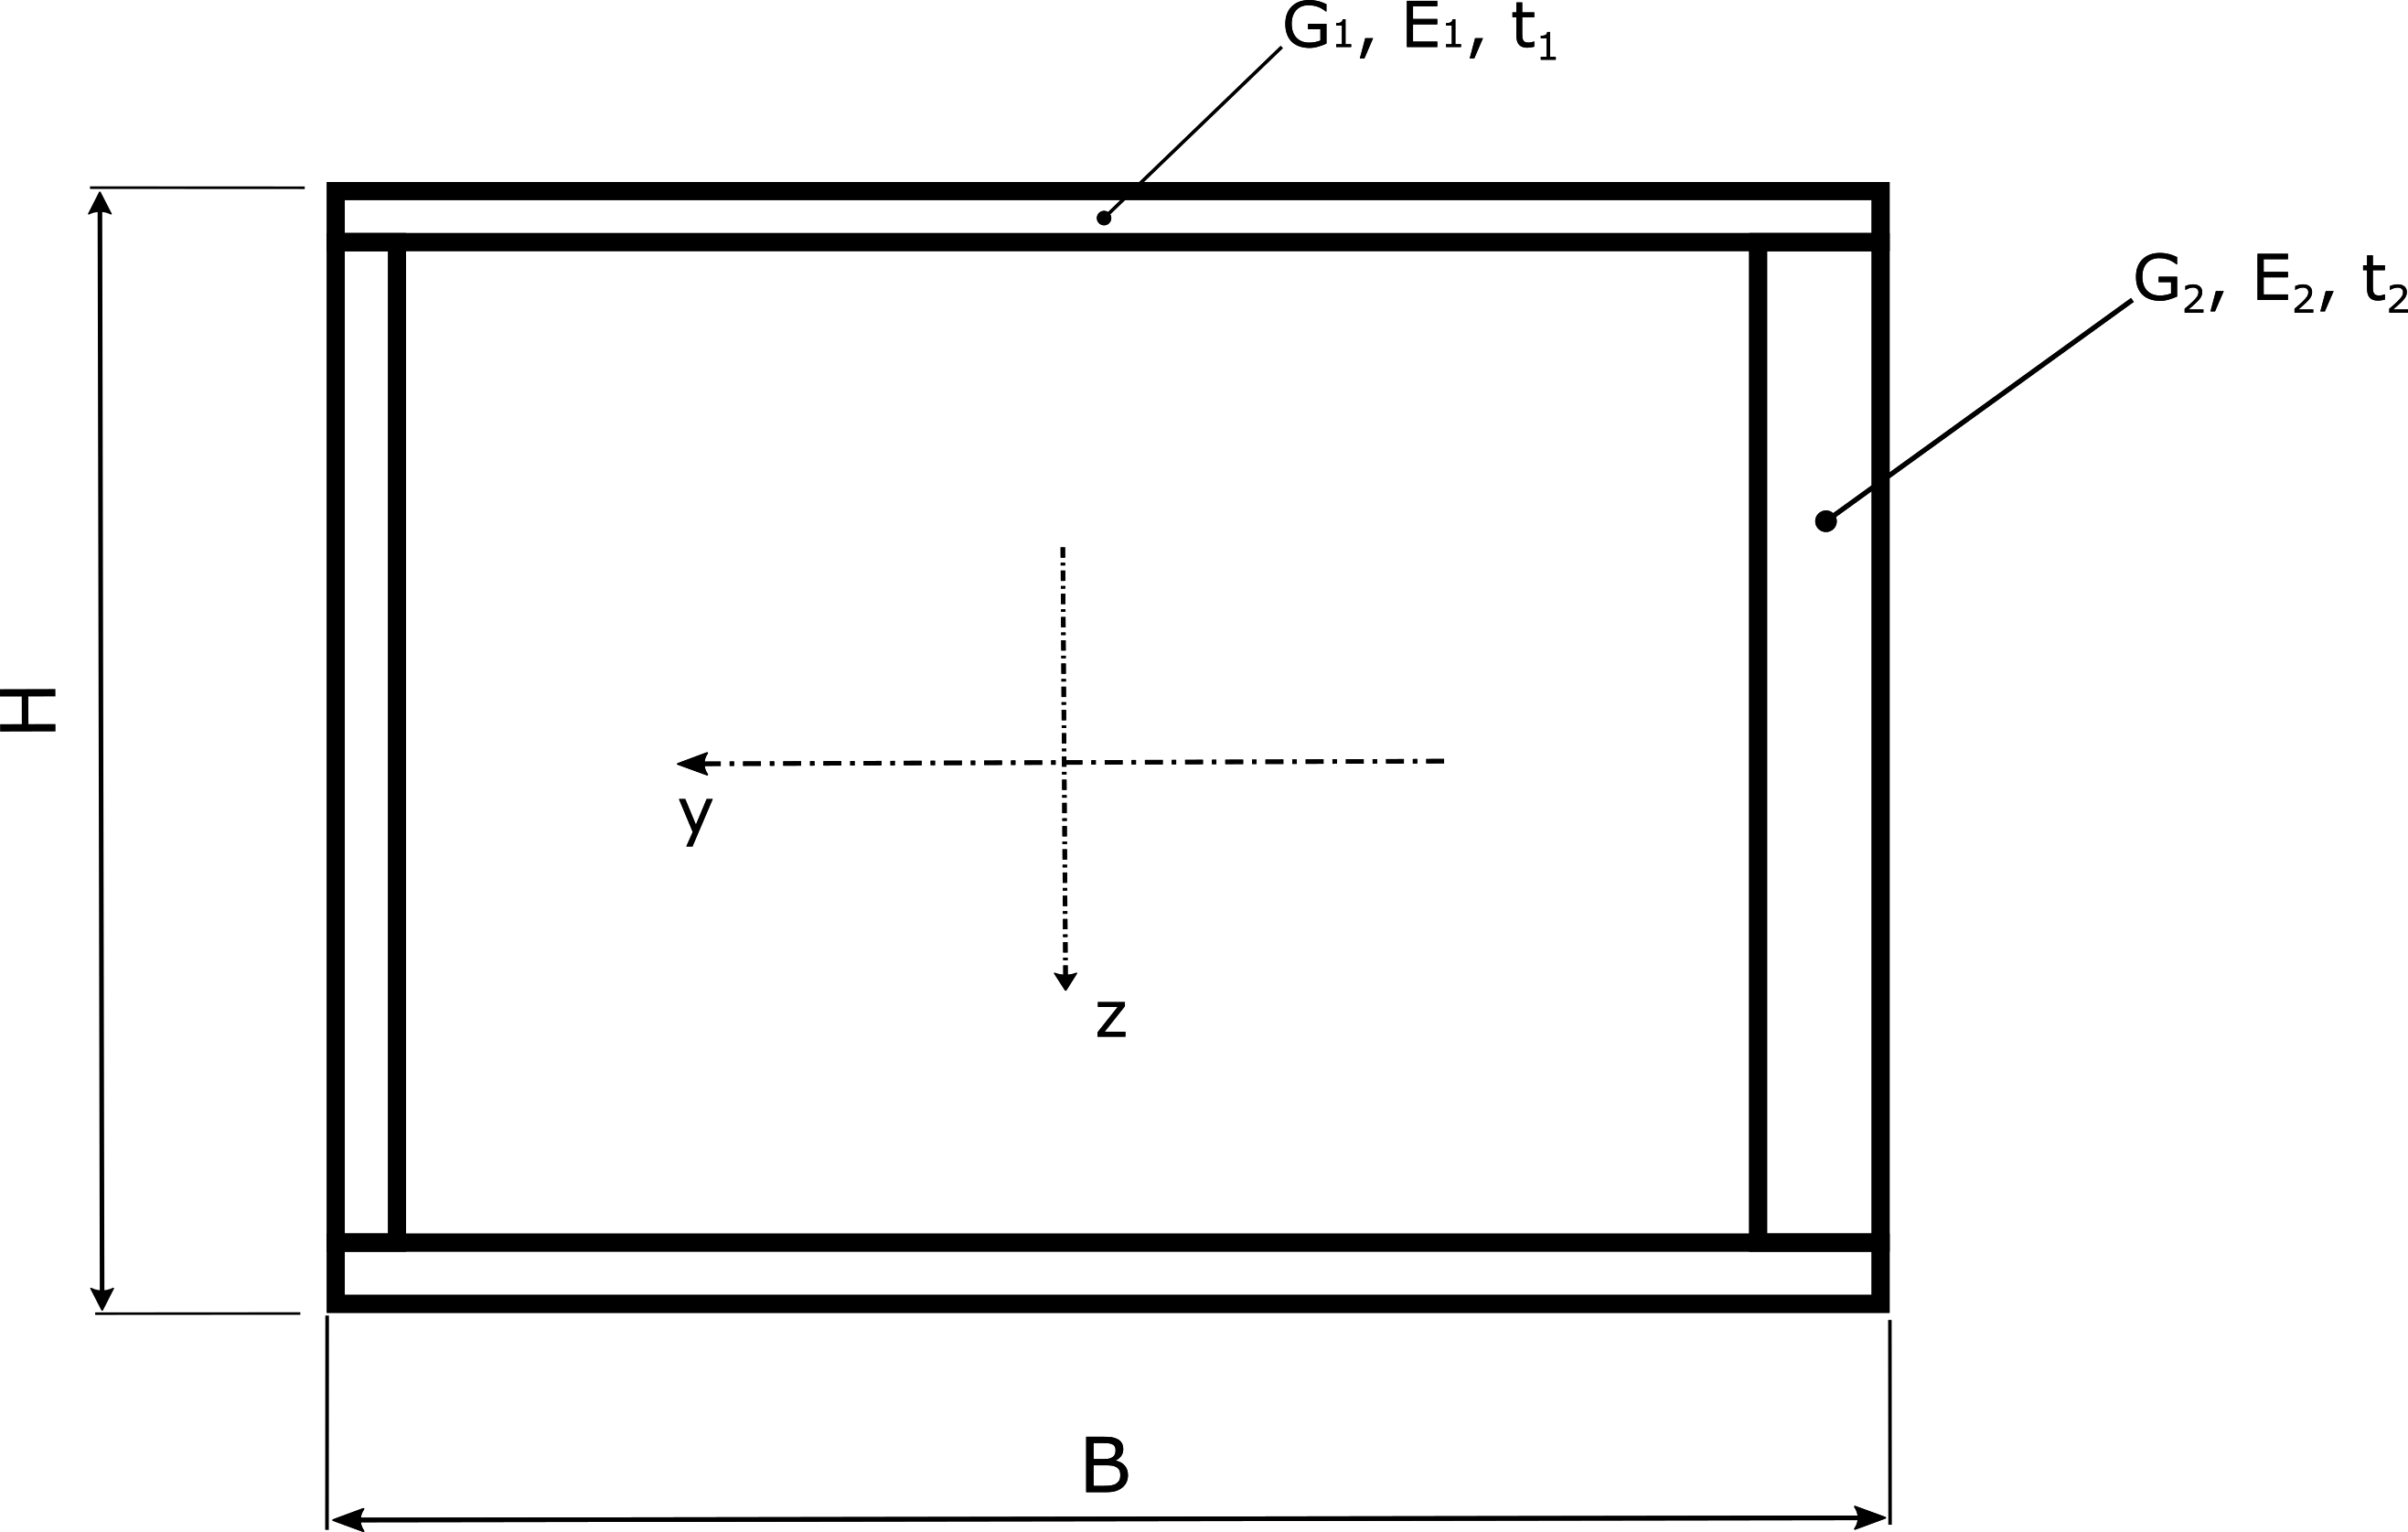
\includegraphics[width=0.7 \textwidth]{model/analyticalBox2}
    \caption[Schematic view of the beam closed section]{Schematic view of the beam closed section. The dimensions are given by the width $B$ and the height $H$. For the upper, lower and left elements, the wall thickness, shear modulus and the Young's modulus are given by $t_1$, $G_1$ and $E_1$, respectively. For the right element, the same parameters are given by $t_2$, $G_2$ and $E_2$.}\label{fig:analyticalBox}
  \end{figure}

  As explained in Section \ref{sec:concept_Model}, the shear stiffness $G_2 t_2$ of the adaptive web can be modified by varying either thickness $t_2$ or shear modulus $G_2$. For the remaining, it is assumed that $t_1 = t_2 = t$ and therefore the thickness $t_2$ is not be considered as a modifiable parameter on the adaptive web.

  Now, the bending-twisting coupling of the structure is investigated using well-known equations to describe the elastic behavior of thin-wall beam elements. Based on the analytical approach to the problem of a beam bending-twisting coupling followed in \cite{Raither2013a}, it is known that warping can be neglected for a configuration like the one presented in this section.

  The bending displacement of the structure is therefore given by Equation \ref{eq:wb}, which a solution of the Bernoulli-Euler equation for a beam:
  %
  \begin{equation}\label{eq:wb}
    w_b = \frac{Q L^3}{6 \Phi_y} \left( -\frac{x^3}{L^3} + \frac{3 x^2}{L^2} \right),
  \end{equation}
  %
  where $w_b$ is the displacement along the $z$ direction and $\Phi_y$ is the flexural stiffness which is given by Equation \ref{eq:flexuralStiffness}:
  %
  \begin{equation}\label{eq:flexuralStiffness}
    \Phi_y = \int \int E(y,z) z^2 \mathrm{d}y \mathrm{d}z.
  \end{equation}

  %Twist
  On the other hand, the twist of a beam with closed section can be obtained from the St. Venant expression for the specific twist $\vartheta$, which is shown in Equation \ref{eq:specificTwist}:
  %
  \begin{equation}\label{eq:specificTwist}
    \vartheta = \frac{\mathrm{d} \phi}{\mathrm{d} x} = \frac{M_t}{4 A_0^2} \oint \frac{\mathrm{d} s}{Gt},
  \end{equation}
  %
  where $A_0$ represent the area enclosed by the profile's wall midline, $\phi$ is the twist of the beam and $M_t$ is the torsional moment applied. Additionally, the torsional stiffness $G I_t$ for the closed section under study is given by the Equation \ref{eq:torStiff}:
  %
  \begin{equation}\label{eq:torStiff}
    G I_t = \frac{4 A_0^2}{\oint \frac{\mathrm{d} s}{G(s) t(s)}}.
  \end{equation}

  In order to calculate the specific twist $\vartheta$ , it is necessary to evaluate the shear centre position $y_{\mathrm{SC}}$ for a given configuration. In order to achieve this, the calculation of the shear flow distribution in the section also needs to be done. To obtain the shear flow $q(s)$, the profile can be considered to be cut at one point, resulting on a opened section. The shear flow $q_{\parallel}(s)$ for this open section case can be calculated using Equation \ref{eq:shearFlowEquation}. The corresponding shear flow for a closed section $q_{\mathrm{C}}$ can be obtained using the Equation \ref{eq:shearFlowDescomposition}:
  %
  \begin{equation}\label{eq:shearFlowEquation}
    q_{\parallel}(s) = - \frac{Q_z}{\Phi_y} S_{E_y}(s),
  \end{equation}
  %
  \begin{equation}\label{eq:shearFlowDescomposition}
    q_{\mathrm{C}}(s) = q_\parallel(s) + q_0,
  \end{equation}
  %
  where $Q_z$ is the force applied in the z direction and $S_{E_y}$ is the so called static moment or first moment of area, which is calculated through the integral shown in Equation \ref{eq:staticMoment}. Also, the variable $q_0$ represents the shear flow at the boundary that results from the torsion of the beam and can be calculated using the Equation \ref{eq:constantShearFlow}:
  %
  \begin{equation}\label{eq:staticMoment}
    S_{E_y}(s) = \int_0^s E(s) t(s) z(s) \mathrm{d}s,
  \end{equation}
  %
  \begin{equation}\label{eq:constantShearFlow}
    q_0 = \frac{Q_z}{\Phi_y} \frac{ \oint_s \frac{S_{E_y}(s)}{G(s) t(s)} \mathrm{d}s }{ \oint_s \frac{1}{G(s) t(s)} \mathrm{d}s }.
  \end{equation}

  Now, the shear centre position in the beam transversal section is calculated for the case of open section. Given that the beam mechanical properties and geometrical dimensions are symmetric around y axis, the shear centre position in the $z$ axis is $z_{\mathrm{SC}} = 0$. On the other hand, the shear centre position in the $y$ axis is given by the Equation \ref{eq:shearCentrePosition}:
  %
  \begin{equation}\label{eq:shearCentrePosition}
    y_{\mathrm{SC,open}} = \frac{1}{Q_z} \oint_s q_\mathrm{C}(s) r(s) \mathrm{d}s,
  \end{equation}
  %
  where $r$ represents the perpendicular distance to the coordinate origin.

  Now, it is necessary that equilibrium exists between the torsional moment due to the shift of the shear centre (caused during the opening of the profile) and the moment due to the torsional shear flow of the closed profile. This condition can be mathematically expressed through Equation \ref{eq:shearCentrePositionMoment}:
  %
  \begin{eqnarray}\label{eq:shearCentrePositionMoment}
  % \nonumber % Remove numbering (before each equation)
    M_\mathrm{t} &=& Q_\mathrm{z} (y_{\mathrm{SC,open}} - y_{\mathrm{SC,closed}}) \nonumber \\
    &=& 2 A_0 q_0.
  \end{eqnarray}
  %
  %where it has been considered that a positive moment $M_\mathrm{t}$ along the x direction produces a constant shear flow distribution which has negative sign given the shear flow distribution definition in the present text.

  The above equality enables on one hand the calculation of the closed section shear centre position $y_{\mathrm{SC,closed}}$ using Equation \ref{eq:closedShearCentre}:
  %
  \begin{equation} \label{eq:closedShearCentre}
    y_{\mathrm{SC,closed}} = y_{\mathrm{SC,open}} - \frac{2 q_0 A0}{Q_z},
  \end{equation}
  %
  and the the calculation of the torsional moment $M_t$ acting on the beam on the other hand using Equation \ref{eq:torMoment}:
  %
  \begin{equation} \label{eq:torMoment}
    M_t = Q_z (y_{\mathrm{load}} - y_{\mathrm{SC,closed}}),
  \end{equation}
  %
  that considers the coordinate $y_{\mathrm{load}}$ of the point where the load is applied.

  Finally, once the torsional moment $M_t$ acting on the beam is known, it is possible to calculate the beam twist $\phi(x)$ using Equation \ref{eq:specificTwist} and considering that $\phi(x) = \vartheta x$.

  %%%%%%%%%%%%% We don't need the total shear flow
  % Finally, the total shear flow $q(s)$ results from the superposition of the shear flow of the open profile $q_\mathrm{C}$ and the constant shear flow due to torsion $q_0$, as shown in the Equation \ref{eq:totalShearFlow}:
  % %
  % \begin{equation}\label{eq:totalShearFlow}
  %   q(s) = q_\mathrm{C}(s) - q_0. %before it was: q_\mathrm{C}(s) - q_\mathrm{M}
  % \end{equation}
  %
\section{Computational model} \label{sec:computationalModel}
  %
  % Description of the model
  %   Include all the parts of the model: C-box shape, inner box, chiral lattice
  %   Figure of the model
  % Parameters included
  %
  % Subsections:
  % - Sub-parts and parametrization of the model, include main dimensions and parameters. Sketch and Abaqus model screenshot
  %     - Lattice
  %     - Lattice nodes with tyre part
  %     - C-box
  %     - Ribs
  % - Attachment points modeling
  % - Parametric study method

  The computational model of the wing box is built using Abaqus CAE commercial software. It consists on three main elements: the wing-box with C-profile, the lattice constituted of the chiral elements and a set of ribs. A general overview of the assembly of the different parts can be seen in Figure \ref{fig:all-assembly}.

  \begin{figure}[!htpb]
    \centering
    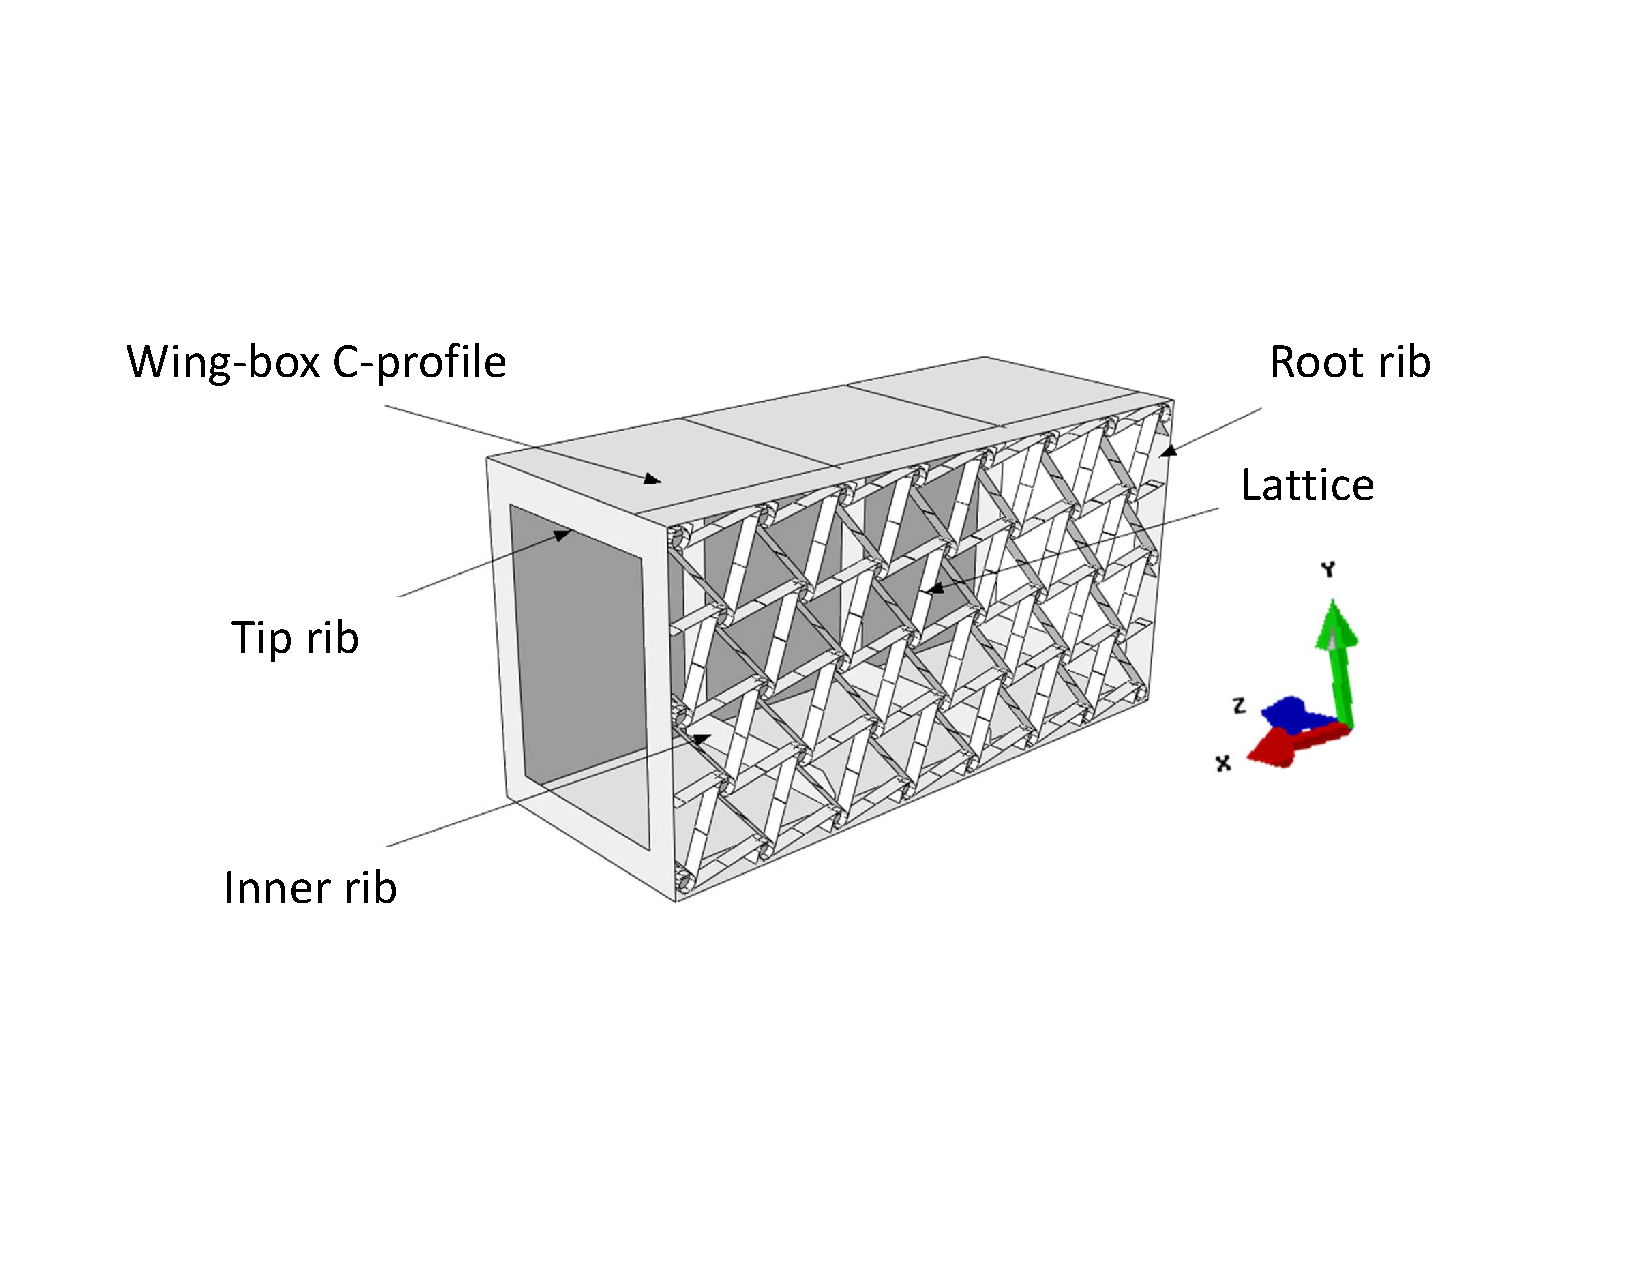
\includegraphics[width=0.8 \textwidth]{model/all-assembly}
    \caption[General assembly configuration for the computational model]{General assembly configuration for the computational model. The different parts for the general configuration include the wing-box profile, the lattice of chiral elements and a set of ribs that can be located at the tip, at the root or in between this borders.}\label{fig:all-assembly}
  \end{figure}

  The discretization of the structural element was done using continuum shell elements as the basic constituting part. An sketch of a continuum shell element as defined in Abaqus can be seen in Figure \ref{fig:shellElement}.

  \begin{figure}[!htpb]
    \centering
    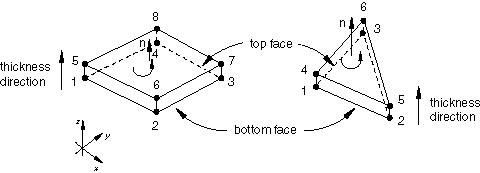
\includegraphics[width=0.8 \textwidth]{model/eshell-scon-normal-nls}
    \caption[Default normals and thickness direction for continuum shell elements in Abaqus]{Default normals and thickness direction for continuum shell elements in Abaqus. \cite{Abaqus}}\label{fig:shellElement}
  \end{figure}

  \subsection{Sub-parts and parametrization of the model} \label{subsec:parametrization_Model}

    \subsubsection{Lattice of chiral elements} \label{subsubsec:lattice_Parametrization}

    The model of the lattice structure is constituted of a network of rigid nodes interconnected by ligaments. At each node, there are six ligaments attached in a uniform distribution that leaves an angular separation of 60$^{\circ}$ between consecutive attachment points. This network constitutes a lattice of chiral elements. An overview of this part can be seen in Figure \ref{fig:lattice}. The lattice structure is divided in an integer number of unit cells in the longitudinal (spanwise) and transversal directions. These parameters are identified with the variables $N$ and $M$ for the longitudinal and transversal directions, respectively. In Figure \ref{fig:lattice-NandM}, an sketch of the internal division for $N = 8$ and $M = 3$ is shown. It displays a set of horizontal rectangles that represent each of the transversal $M$ divisions while the set of vertical rectangles correspond to each of the $N$ longitudinal divisions.

    \begin{figure}[!htpb]
      \centering
      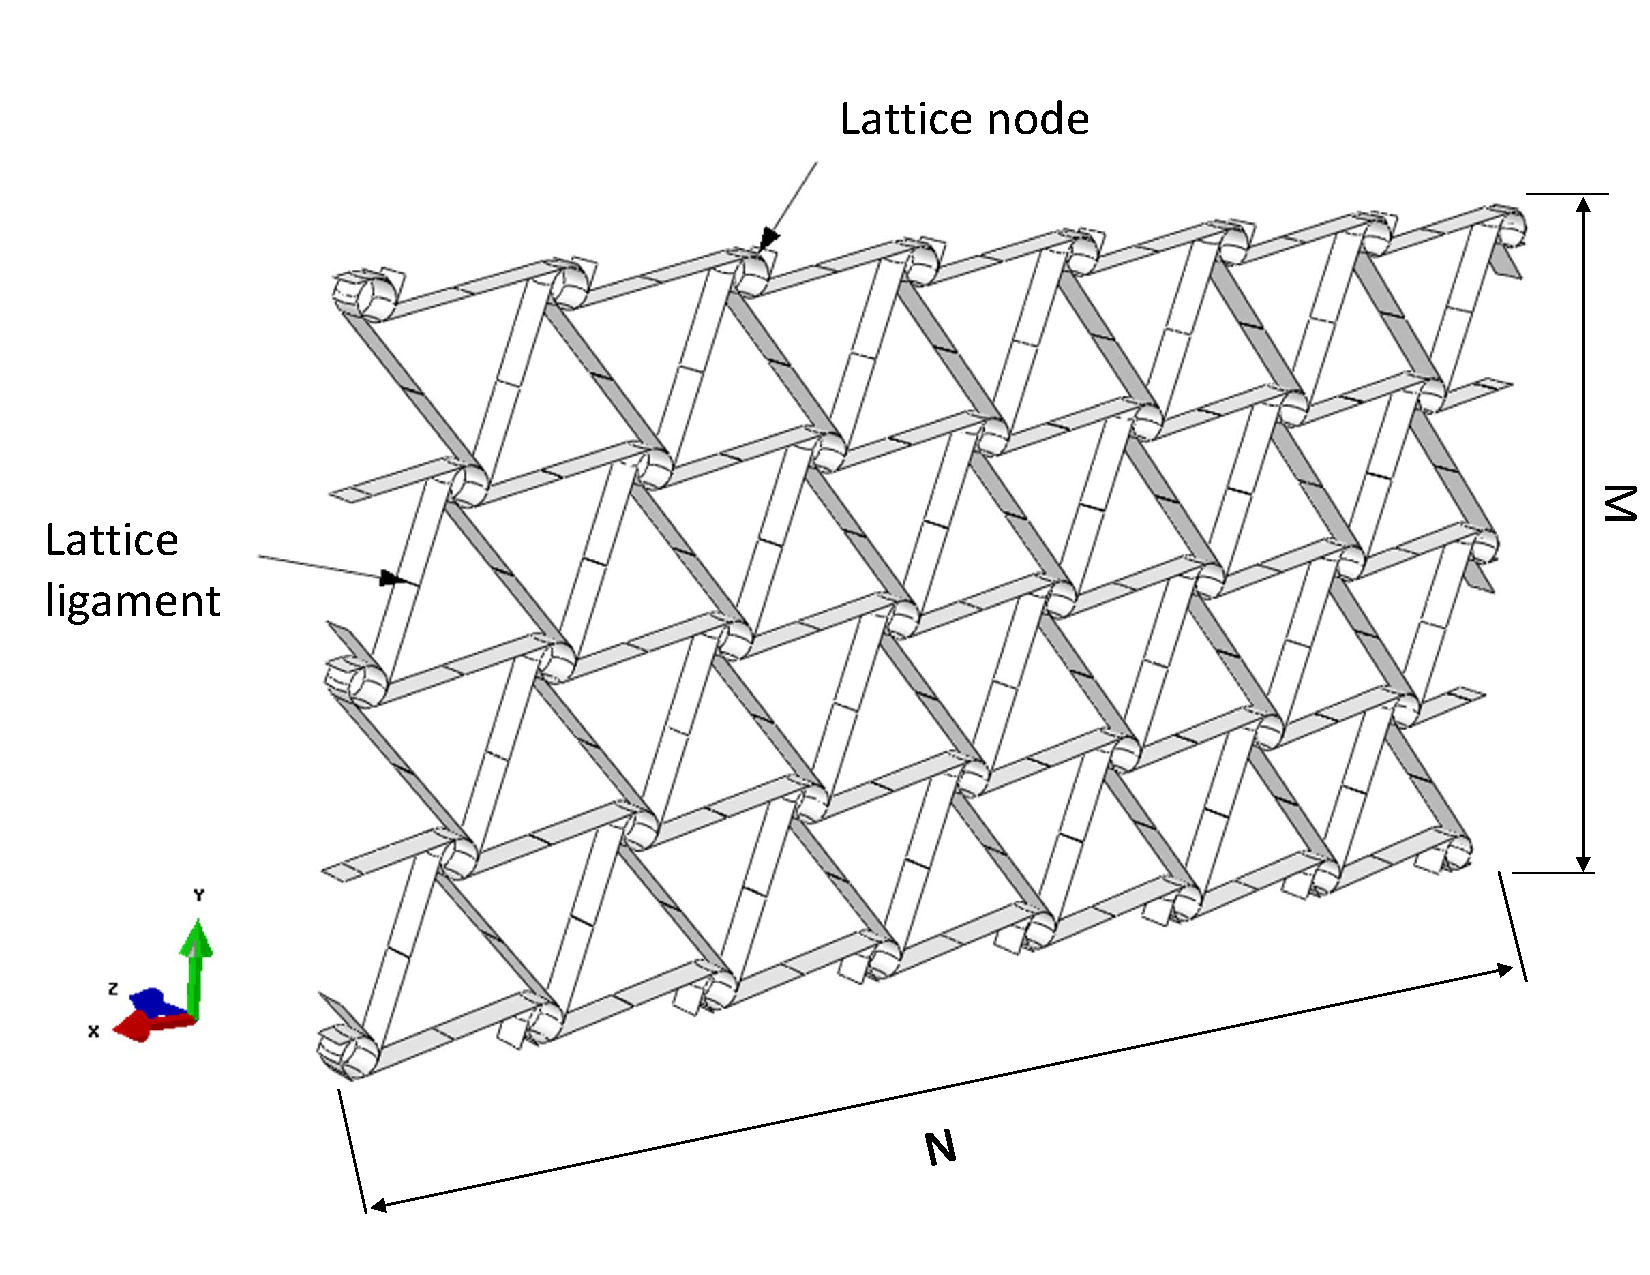
\includegraphics[width=0.8 \textwidth]{model/lattice}
      \caption[Overview of the lattice of chiral elements part]{Overview of the lattice of chiral elements part. The parameters $N$ and $M$ represent the number of unit cells in the longitudinal (spanwise) and transversal directions, respectively.}\label{fig:lattice}
    \end{figure}

    \begin{figure}[!htpb]
      \centering
      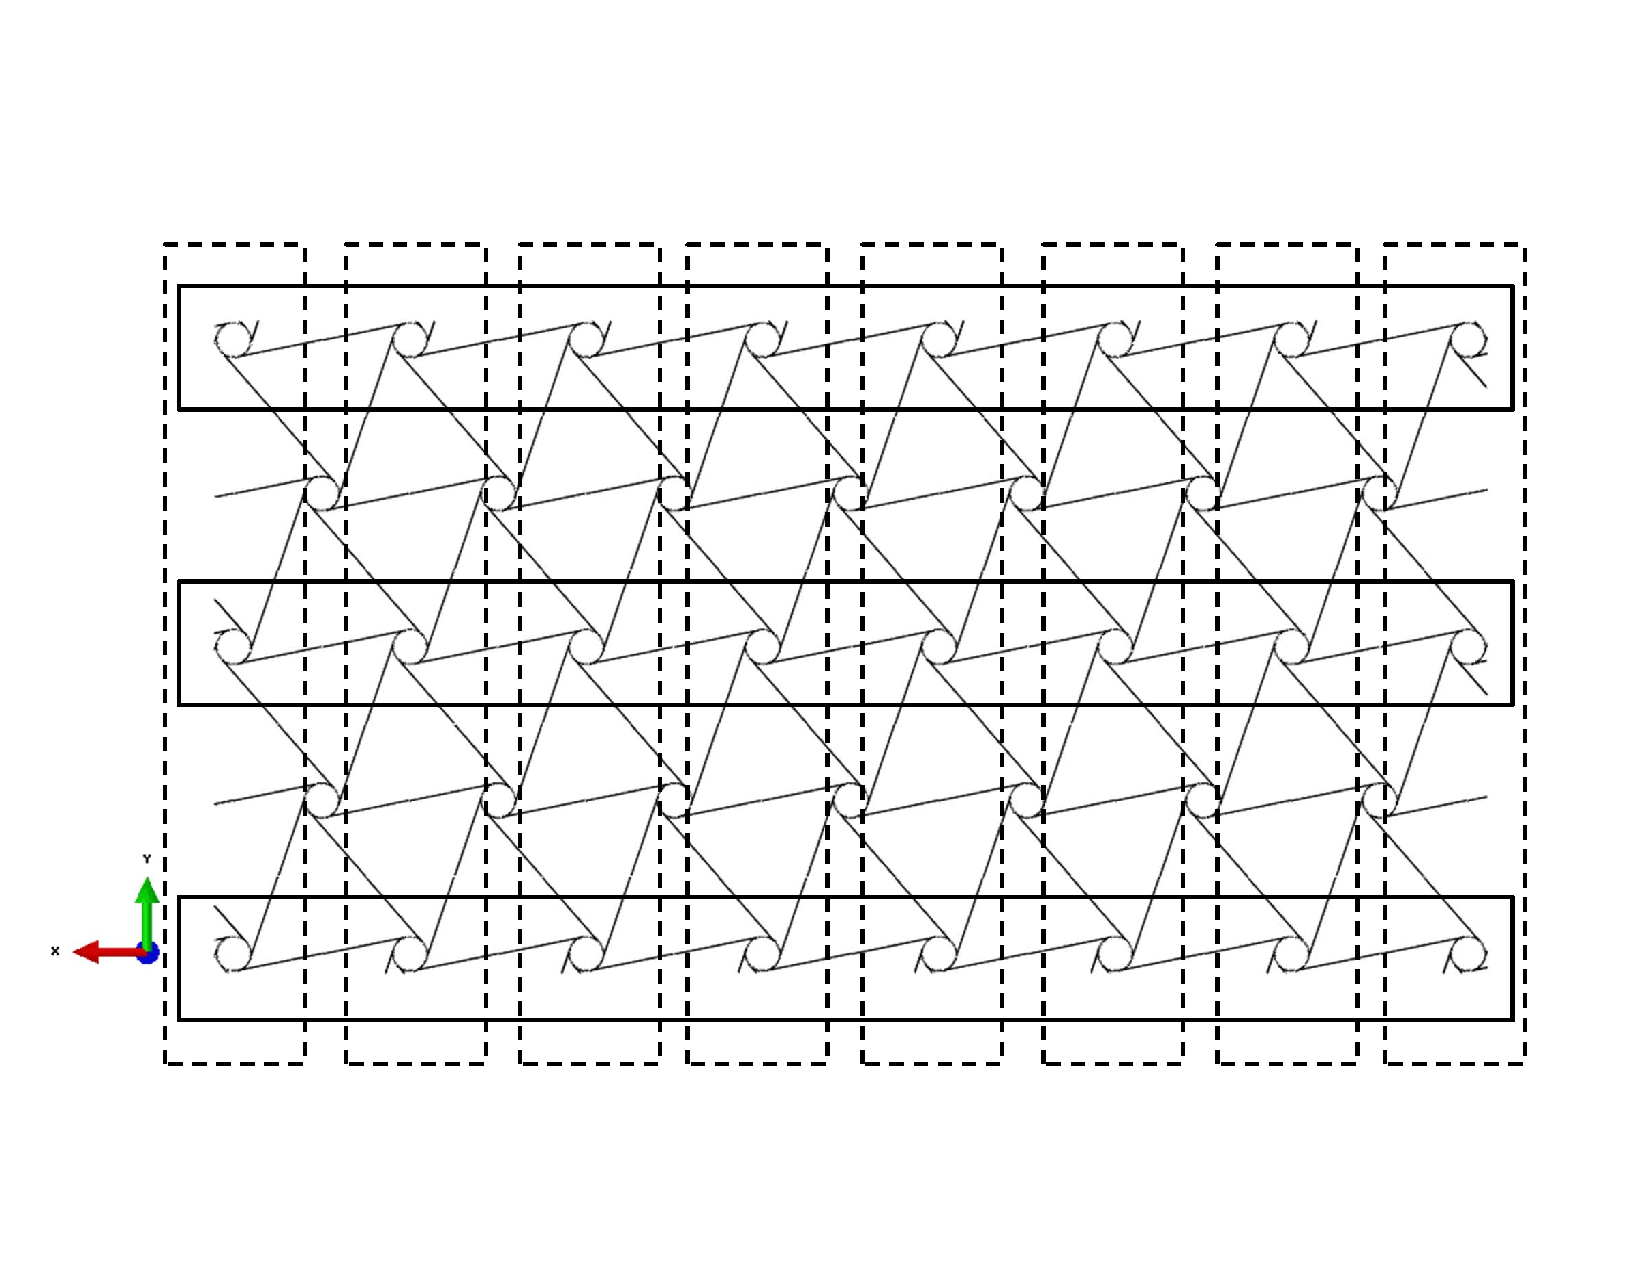
\includegraphics[width=0.8 \textwidth]{model/lattice-NandM}
      \caption[Division of the lattice structure in cell units]{Division of the lattice structure in cell units. The sketch shows a lattice with $N = 8$ and $M = 3$. The set of horizontal rectangles represent each of the transversal $M$ divisions while the set of vertical rectangles correspond to each of the $N$ longitudinal divisions.}\label{fig:lattice-NandM}
    \end{figure}

    \clearpage
    Furthermore, the internal geometry in the chiral structure is determined by a number of parameters: the thickness $t_{\mathrm{chi}}$, the ligament eccentricity $e_{\mathrm{chi}}$, the ligament half length $L_{\mathrm{chi}}$, the lattice node depth $B_{\mathrm{chi}}$ and the lattice node radius $r_{\mathrm{chi}}$. The geometrical meaning of these variables can be seen in the sketch shown in Figure \ref{fig:lattice-internalParameters}. The thickness $t_{\mathrm{chi}}$ applies for both the ligaments and the lattice nodes geometries. The eccentricity $e_{\mathrm{chi}}$ is expressed as the dimensionless parameter $\epsilon_{\mathrm{chi}}$ which is obtained from $\epsilon_{\mathrm{chi}} = e_{\mathrm{chi}} / B_{\mathrm{chi}}$.

    In the sketch shown in Figure \ref{fig:lattice-internalParameters} an additional dimension variable appears, the ligament eccentricity radius $R_{\mathrm{chi}}$ which is dependent on the ligament eccentricity $e_{\mathrm{chi}}$ and the lattice node depth $B_{\mathrm{chi}}$ as shown in Equation \ref{eq:RforLattice}.

    A summary of all the parameters introduced to characterize the chiral lattice structure together with their units and nominal values is shown in Table \ref{tab:parameters_lattice}.

    \begin{equation}\label{eq:RforLattice}
      R = \frac{e_{\mathrm{chi}}^2 + \frac{B_{\mathrm{chi}}^2}{4}}{2e_{\mathrm{chi}}}
    \end{equation}

    \begin{figure}[!htpb]
      \centering
      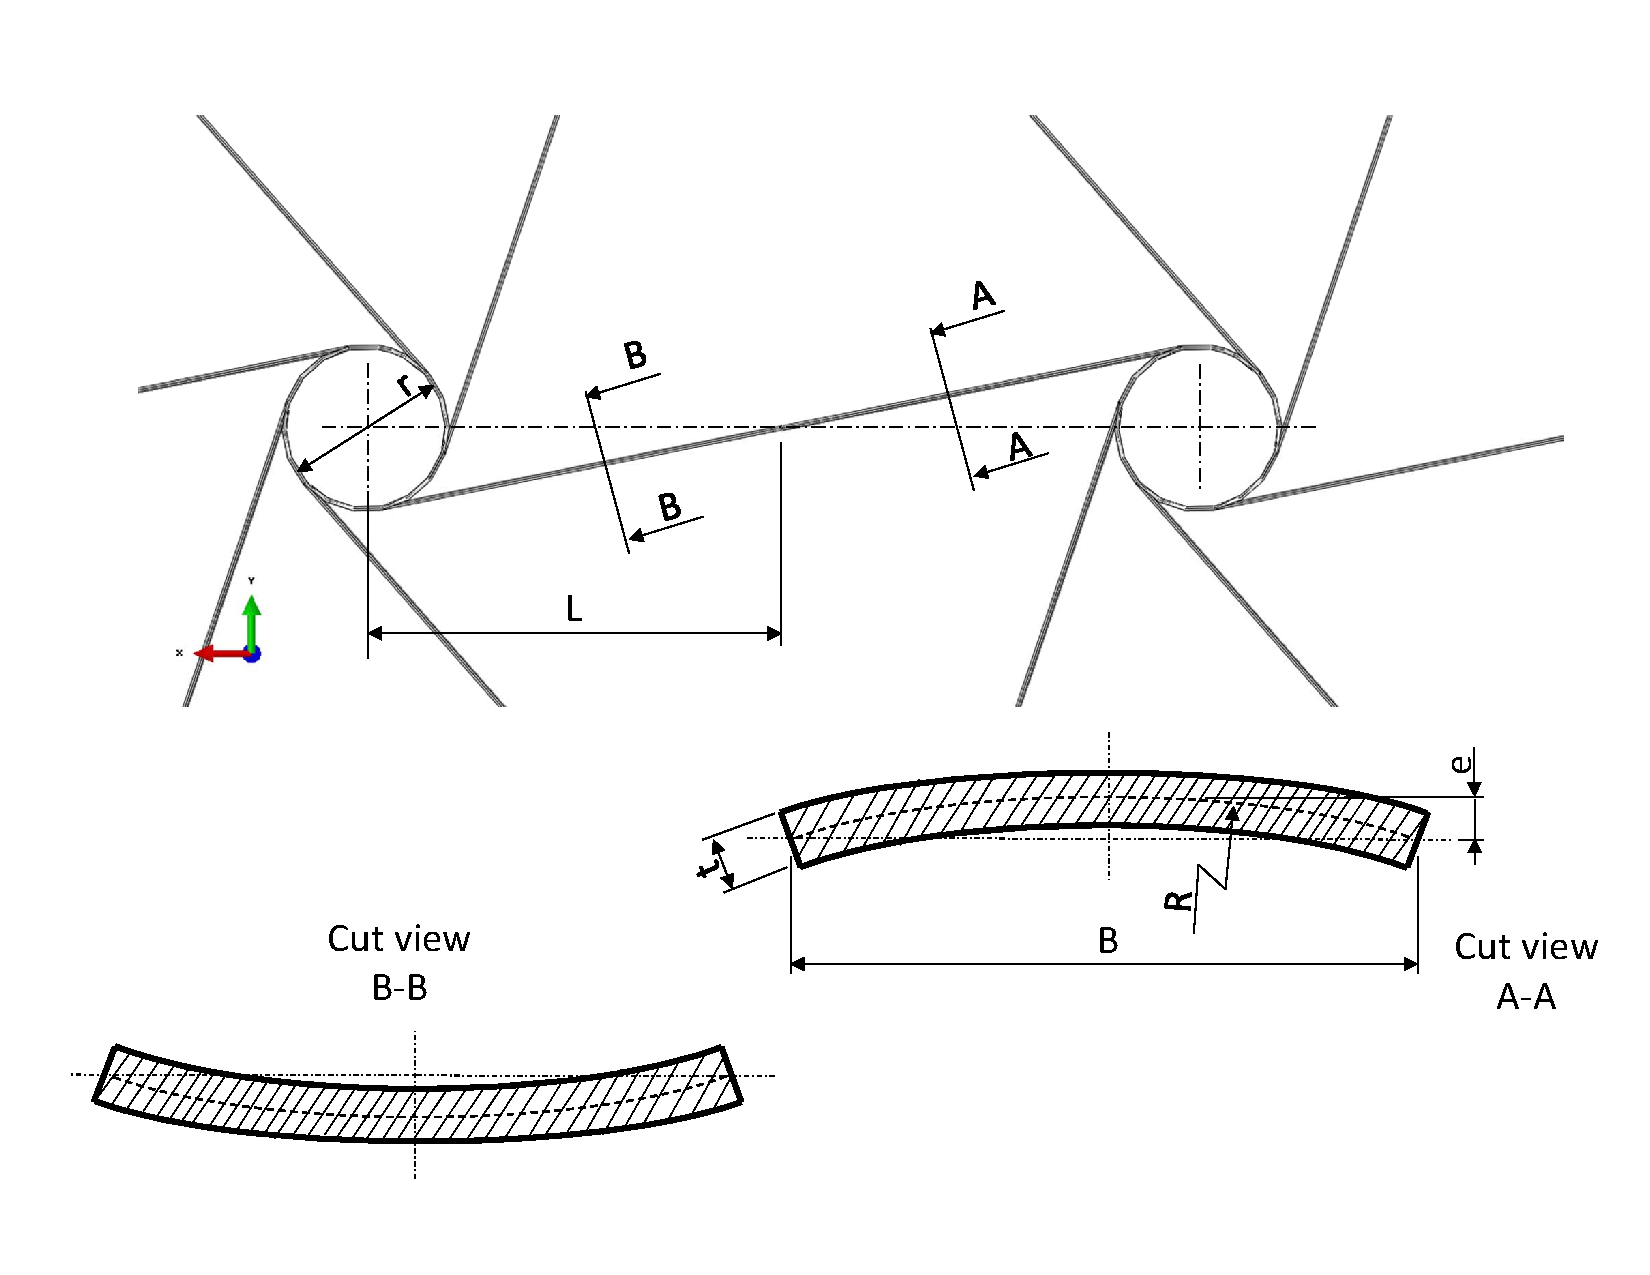
\includegraphics[width=0.8 \textwidth]{model/lattice-internalParameters}
      \caption[Internal parameters of the chiral structure in the lattice]{Internal parameters of the chiral structure in the lattice. The geometry is characterized by the the ligament eccentricity $e_{\mathrm{chi}}$, the ligament half length $L_{\mathrm{chi}}$, the lattice node depth $B_{\mathrm{chi}}$, the lattice node radius $r_{\mathrm{chi}}$ and the thickness $t_{\mathrm{chi}}$. The ligament eccentricity radius $R_{\mathrm{chi}}$ which is dependent on the ligament eccentricity $e_{\mathrm{chi}}$ and the lattice node depth $B_{\mathrm{chi}}$, as shown in Equation \ref{eq:RforLattice}}\label{fig:lattice-internalParameters}
    \end{figure}

    \begin{table}[!htpb]
    \centering
    \begin{tabular}{|l|lll|}
    \hline
    \textbf{Parameter} & \multicolumn{1}{l|}{\textbf{Symbol}} & \multicolumn{1}{l|}{\textbf{Units}} & \textbf{Nominal value} \\ \hline \hline
    {\textbf{Dimensions}} &  &  &  \\ \hline
    Number of unit cells in spanwise direction & \multicolumn{1}{l|}{$N$} & \multicolumn{1}{l|}{} & 8 \\ \hline
    Number of unit cells in transversal direction & \multicolumn{1}{l|}{$M$} & \multicolumn{1}{l|}{} & 3 \\ \hline
    Dimensionless ligament eccentricity (e/B) & \multicolumn{1}{l|}{$\epsilon_{\mathrm{chi}}$} & \multicolumn{1}{l|}{} & 0.01 \\ \hline
    Node radius & \multicolumn{1}{l|}{$r_{\mathrm{chi}}$} & \multicolumn{1}{l|}{mm} & 10 \\ \hline
    Node depth & \multicolumn{1}{l|}{$B_{\mathrm{chi}}$} & \multicolumn{1}{l|}{mm} & 20 \\ \hline
    Ligament eccentricity radius & \multicolumn{1}{l|}{$R_{\mathrm{chi}}$} & \multicolumn{1}{l|}{mm} & 250.1 \\ \hline
    Ligament half length & \multicolumn{1}{l|}{$L_{\mathrm{chi}}$} & \multicolumn{1}{l|}{mm} & 50 \\ \hline
    Thickness & \multicolumn{1}{l|}{$t_{\mathrm{chi}}$} & \multicolumn{1}{l|}{mm} & 0.5 \\ \hline \hline
    {\textbf{Material (ABS)}} &  &  &  \\ \hline
    Young's modulus & \multicolumn{1}{l|}{$E_{\mathrm{chi}}$} & \multicolumn{1}{l|}{N/mm$^2$} & 3100 \\ \hline
    Poisson's ratio & \multicolumn{1}{l|}{$\nu_{\mathrm{chi}}$} & \multicolumn{1}{l|}{} & 0.3 \\ \hline
    \end{tabular}
    \caption[Parameters used for the lattice model]{Parameters used for the lattice model. The mechanical properties of the material used correspond to ABS, which is a common thermoplastic polymer.}
    \label{tab:parameters_lattice}
    \end{table}

    \clearpage
    \subsubsection{Wing-box in C-profile} \label{subsubsec:wingBox_Parametrization}

    %Description of the wing box
    The model of the wing-box consists on a beam with open C profile. The length $L_{\mathrm{box}}$ and height $H_{\mathrm{box}}$ of the part are determined from those of the lattice of chiral elements. Therefore, the tailorable parameters for this part are the width $W_{\mathrm{box}}$, the thickness $t_{\mathrm{box}}$ and the mechanical properties $E_{\mathrm{box}}$ and $\nu_{\mathrm{box}}$ of the material used.

    \begin{figure}[!htpb]
      \centering
      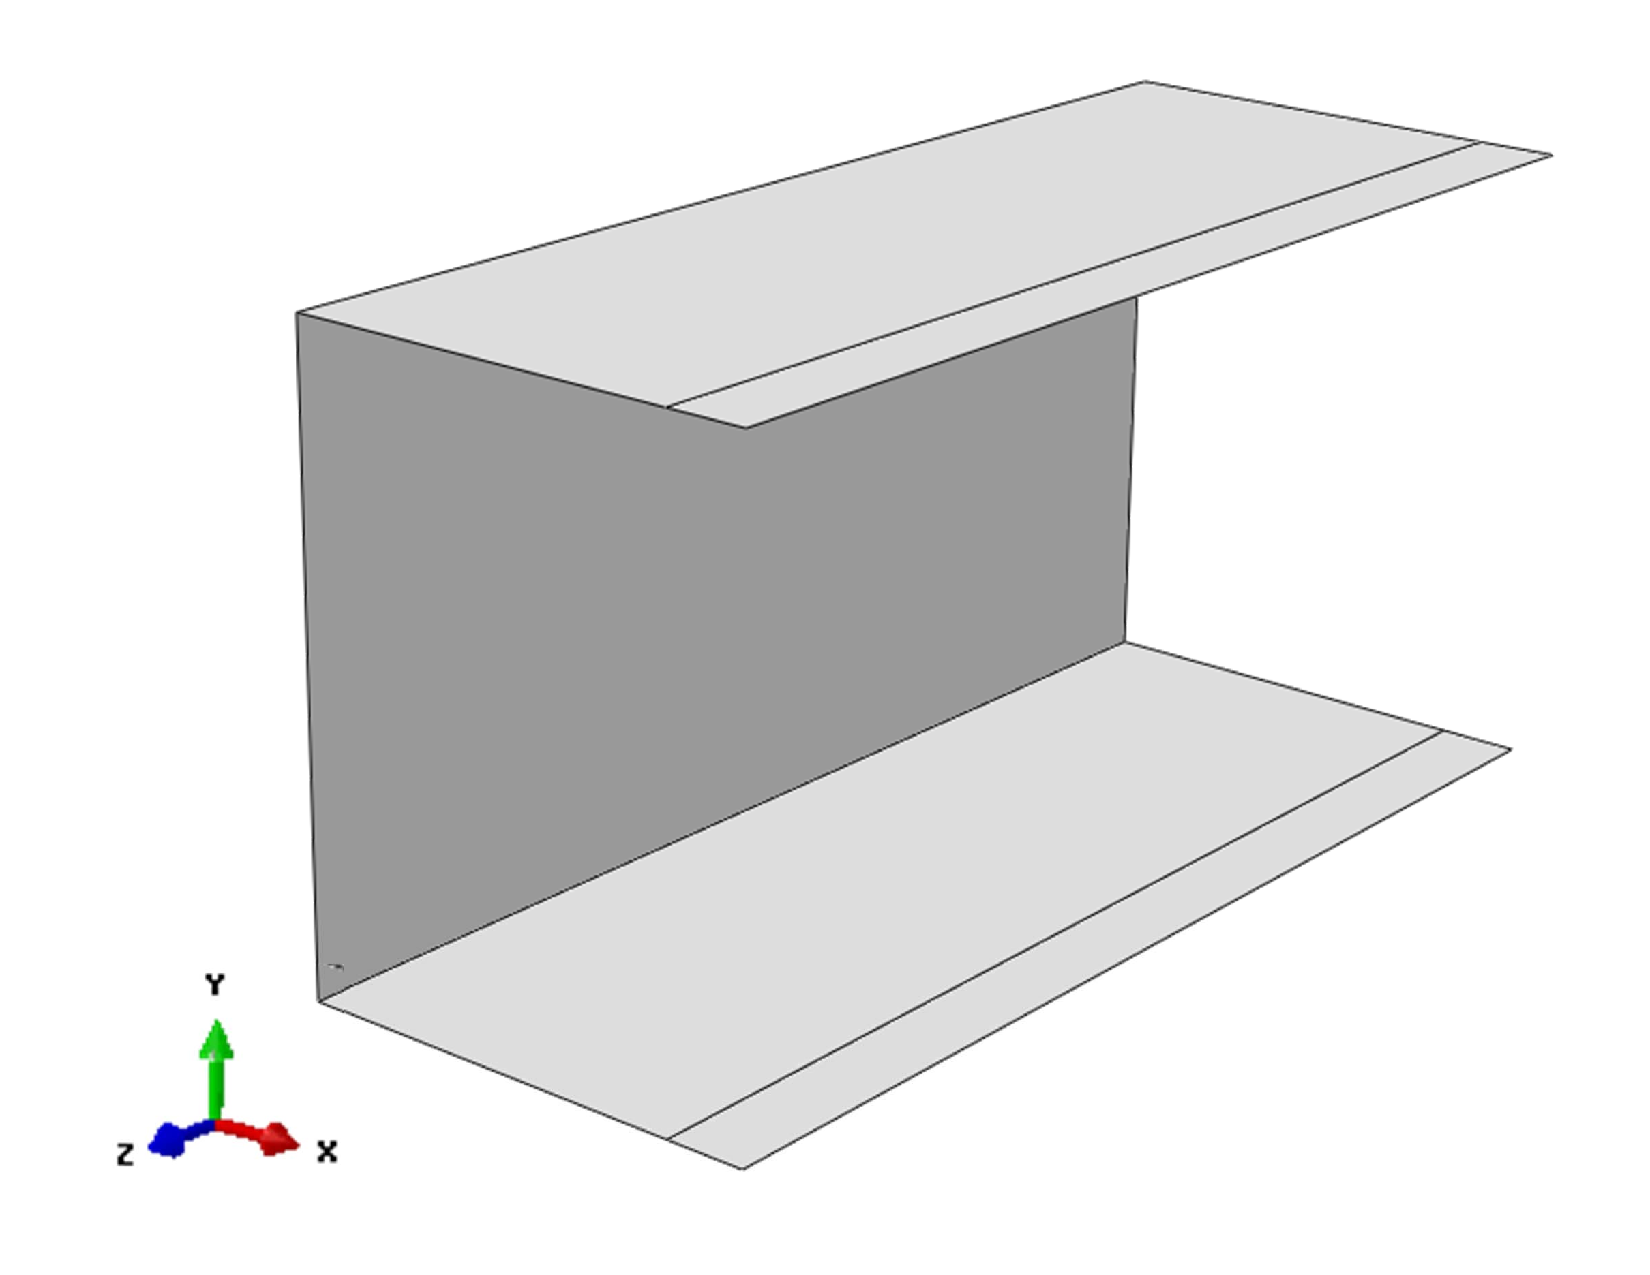
\includegraphics[width=0.6 \textwidth]{model/wing-box}
      \caption[Overview of the wing-box in C-profile part]{Overview of the wing-box in C-profile part}\label{fig:wing-box}
    \end{figure}

    In the sketch shown in Figure \ref{fig:wing-box-internalParameters} it is possible see the geometrical meaning of the parameters introduced in the previous paragraph. Additionally, the Table \ref{tab:parameters_wing-box} shows its units and nominal values.

    \begin{figure}[!htpb]
      \centering
      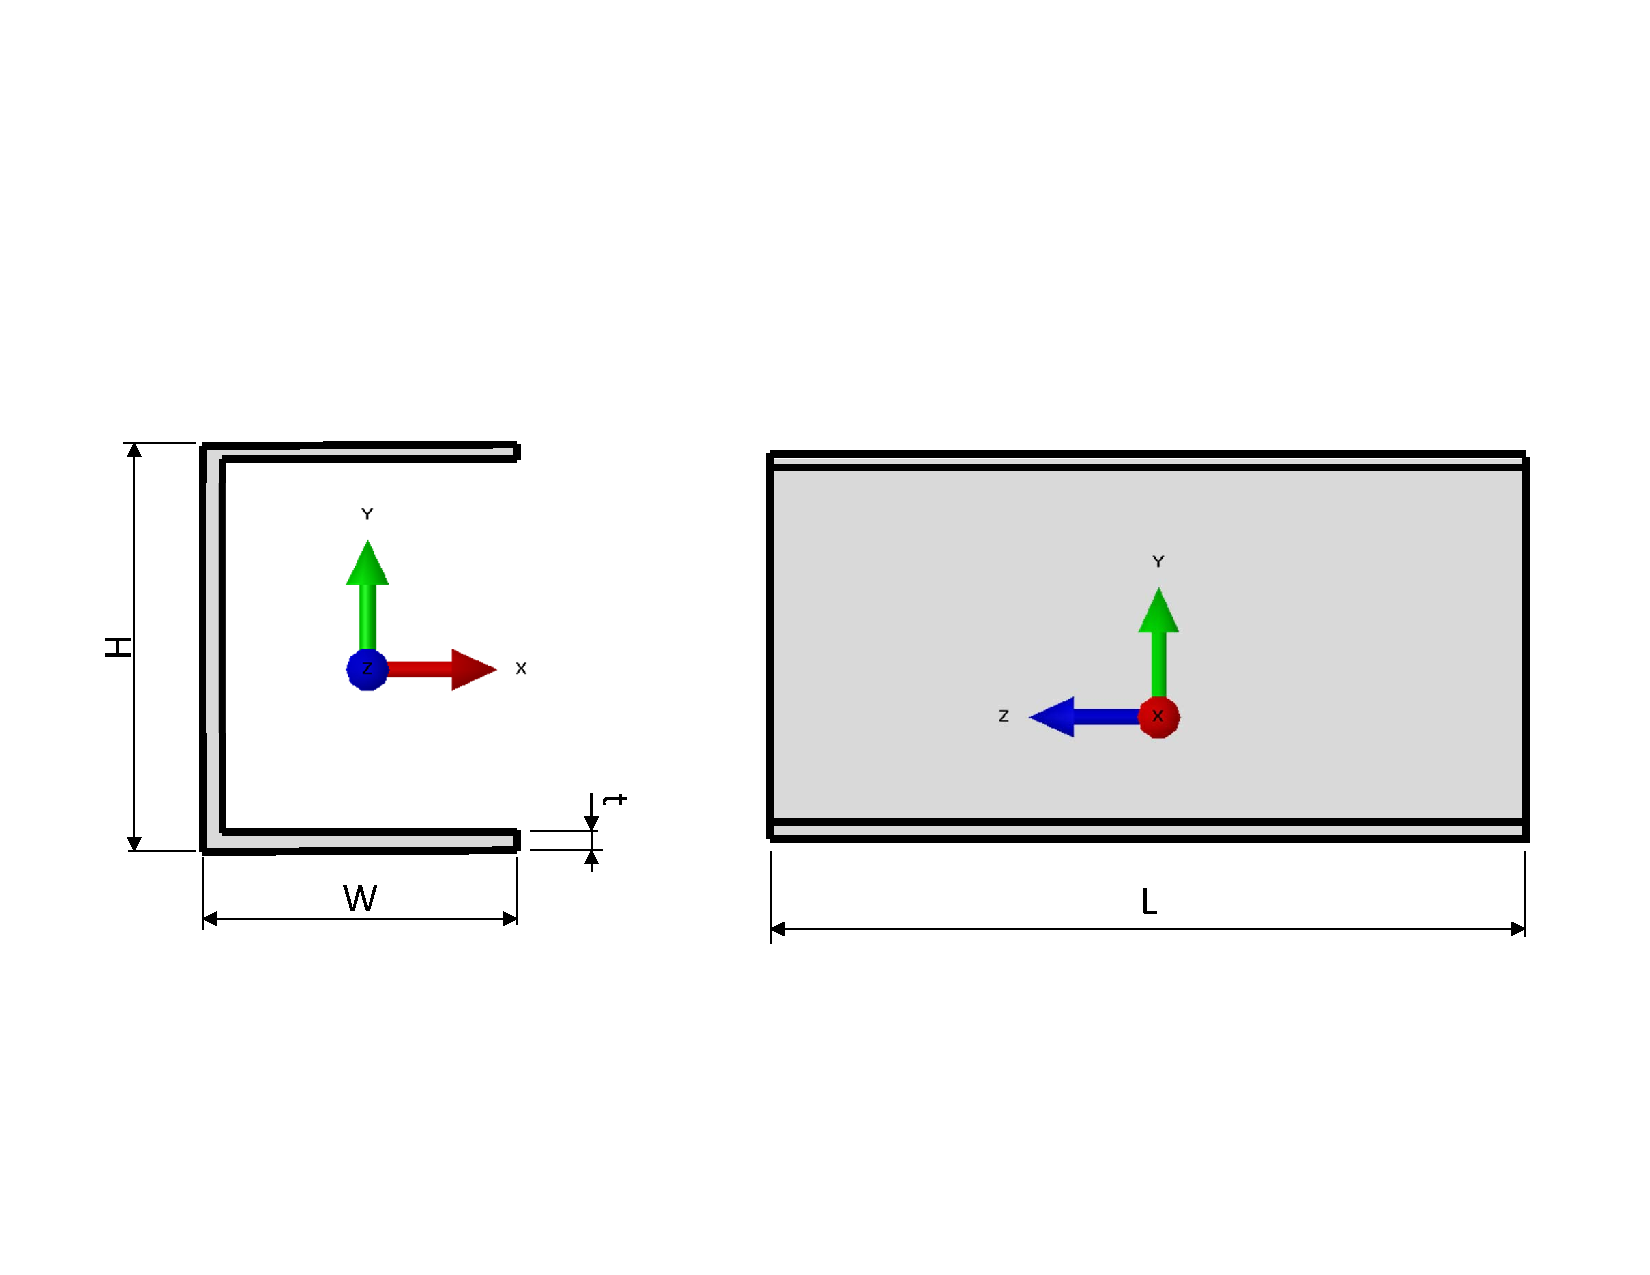
\includegraphics[width=0.8 \textwidth]{model/wing-box-internalParameters}
      \caption[Internal parameters of the wing-box in C-profile part]{Internal parameters of the wing-box C-profile part. The geometry of the part is determined by the length $L_{\mathrm{box}}$, height $H_{\mathrm{box}}$, the width $W_{\mathrm{box}}$ and the thickness $t_{\mathrm{box}}$.}\label{fig:wing-box-internalParameters}
    \end{figure}

    \begin{table}[!htpb]
    \centering
    \begin{tabular}{|l|lll|}
    \hline
    \textbf{Parameter} & \multicolumn{1}{l|}{\textbf{Symbol}} & \multicolumn{1}{l|}{\textbf{Units}} & \textbf{Nominal value} \\ \hline \hline
    {\textbf{Dimensions}} &  &  &  \\ \hline
    Wing-box height & \multicolumn{1}{l|}{$H_{\mathrm{box}}$} & \multicolumn{1}{l|}{mm} & 383.27 \\ \hline
    Wing-box length & \multicolumn{1}{l|}{$L_{\mathrm{box}}$} & \multicolumn{1}{l|}{mm} & 743.86 \\ \hline
    Wing-box width & \multicolumn{1}{l|}{$W_{\mathrm{box}}$} & \multicolumn{1}{l|}{mm} & 300 \\ \hline
    Wing-box thickness & \multicolumn{1}{l|}{$t_{\mathrm{box}}$} & \multicolumn{1}{l|}{mm} & 0.8 \\ \hline \hline
    {\textbf{Material (Aluminum)}} &  &  &  \\ \hline
    Young's modulus & \multicolumn{1}{l|}{$E_{\mathrm{box}}$} & \multicolumn{1}{l|}{N/mm$^2$} & 69000 \\ \hline
    Poisson's ratio & \multicolumn{1}{l|}{$\nu_{\mathrm{box}}$} & \multicolumn{1}{l|}{} & 0.3269 \\ \hline
    \end{tabular}
    \caption[Parameters used for the wing-box in C-profile model]{Parameters used for the wing-box in C-profile model. The mechanical properties of the material used correspond to standard aluminum. The value of the wing-box height $H_{\mathrm{box}}$ and the wing-box length $L_{\mathrm{box}}$ are not independent but are calculated based on the transversal and longitudinal dimensions of the chiral lattice structure, respectively.}
    \label{tab:parameters_wing-box}
    \end{table}

    \clearpage
    \subsubsection{Ribs} \label{subsubsec:Ribs_Parametrization}

    In order to provide the wing-box with additional stiffness in the transversal direction, the addition of ribs is considered. For its design, two different approaches are studied. One considers a open profile design while the other considers a close profile design, as shown in Figure \ref{fig:rib-internalParameters}. These could be installed at the tip and/or root of the wing box; and also, in the interior of the wing-box. For those ribs located in this last position, the open section design is preferred to avoid interferences with the lattice of chiral structures. For the ribs located in an outer position, considerations regarding the optimal design choice will be presented in Subsection \ref{subsec:ribs_results_model}.

    The ribs design is characterized by the widths $W_{\mathrm{rib,close}}$ and $W_{\mathrm{rib,open}}$, and the height $H_{\mathrm{rib}}$. The height $H_{\mathrm{rib}}$ and the width of the closed section design $W_{\mathrm{rib,close}}$ are set to be equal to those of the wing-box: $H_{\mathrm{rib}} = H_{\mathrm{box}}$ and $W_{\mathrm{rib}} = W_{\mathrm{rib,close}}$, respectively. The value of $W_{\mathrm{rib,open}}$ is calculated as follows:
    \begin{equation*}
    W_{\mathrm{rib,open}} = B_{\mathrm{chi}} + W_{\mathrm{rib,close}} + d_{\mathrm{chi-rib}}
    \end{equation*}
    where $d_{\mathrm{chi-rib}}$ represents the gap between the right edges of the inner rib and the lattice chiral structure. This gap ensures that there are not any interferences in between the rib and the lattice chiral structure. The value of this parameter was set to a fix value of $d_{\mathrm{chi-rib}} = 20$mm. Additionally, the frame width $A_{\mathrm{rib}}$ and the thickness $t_{\mathrm{rib}}$ allow design modifications.

    \begin{figure}[!htpb]
      \centering
      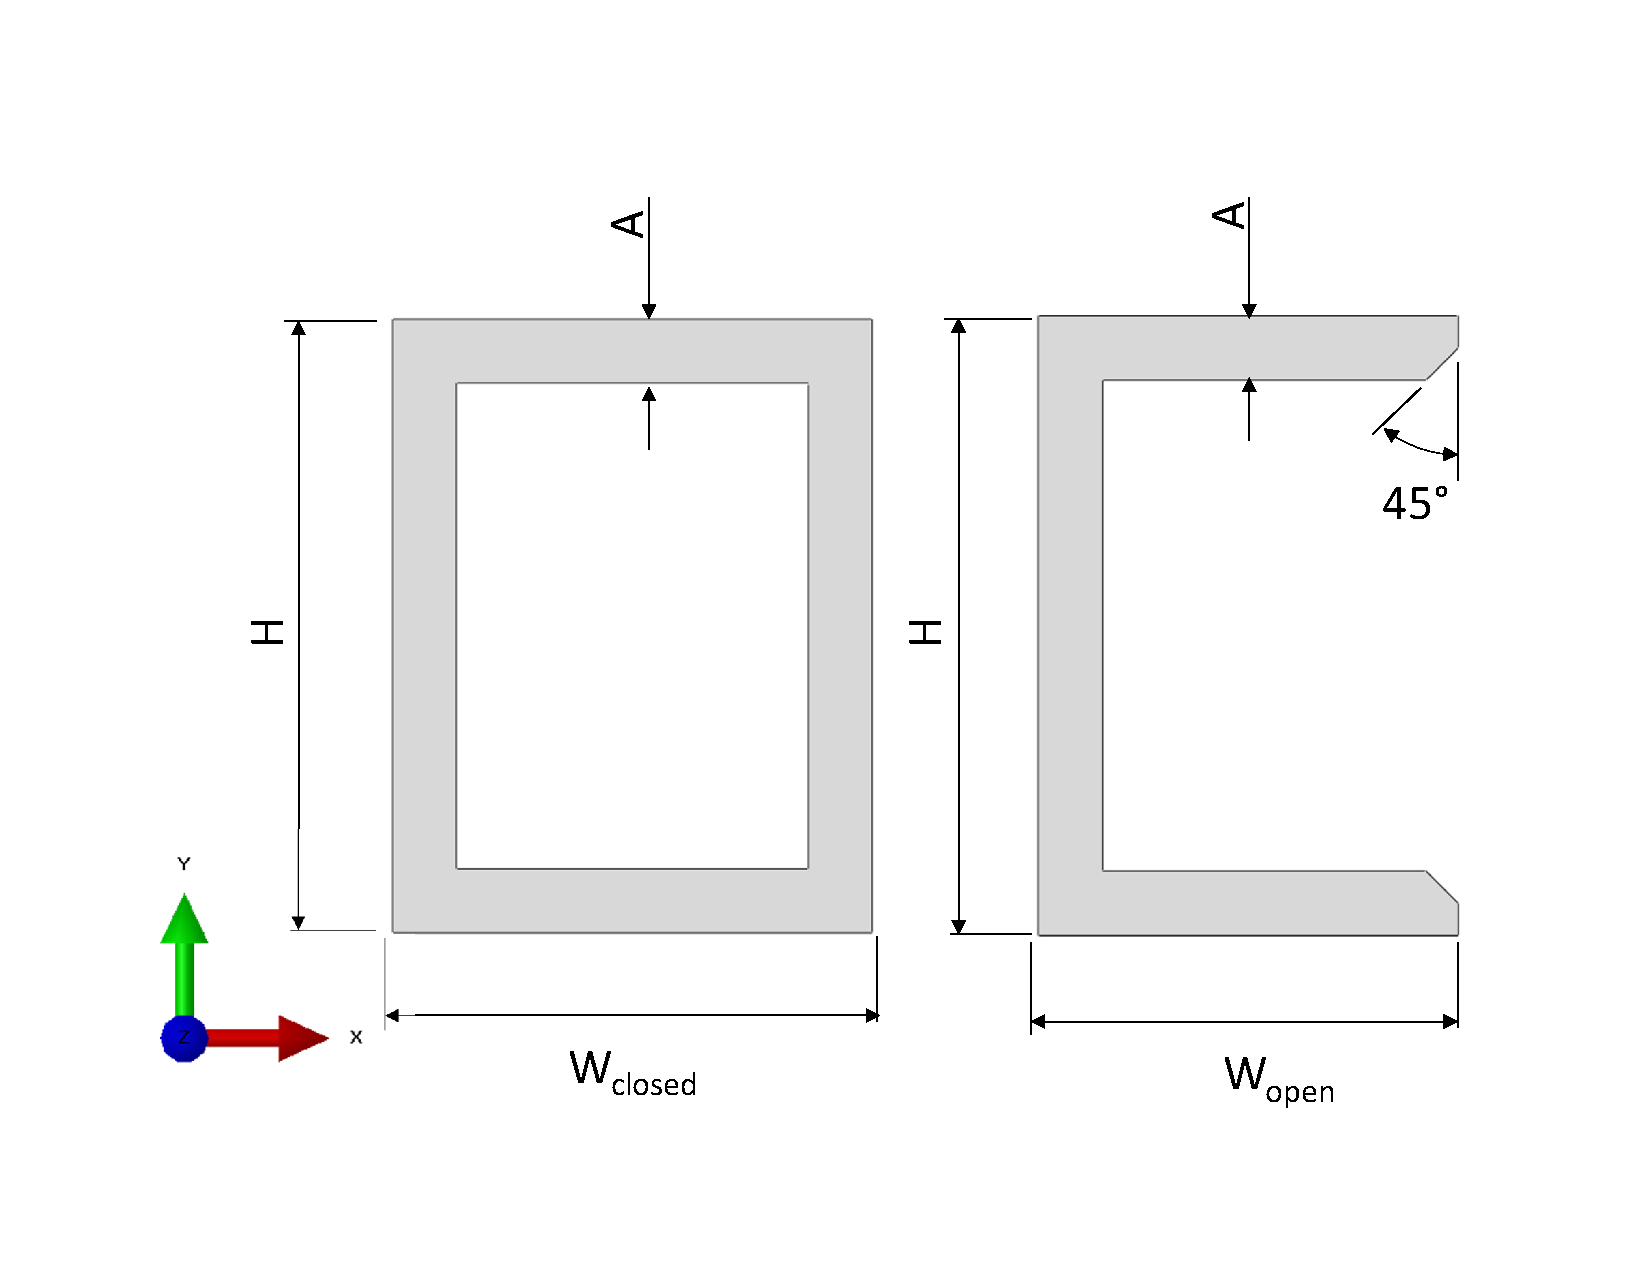
\includegraphics[width=0.8 \textwidth]{model/rib-internalParameters}
      \caption[Internal parameters of the two different ribs parts]{Internal parameters of the two different ribs parts. The angle edge for the open section configuration is set to a fix value of 45$^{\circ}$ to simplify the design and assuming this area of the rib is not critical for the rib duty. }\label{fig:rib-internalParameters}
    \end{figure}

    The nominal values of all the parameters involved in the ribs design can be read in Table \ref{tab:parameters_rib}. The material choice aimed for a configuration stiffer than the wing-box to ensure no out-of-plane deformation of the rib. For this reason, the material chosen is steel.

    \begin{table}[!htpb]
    \centering
    \begin{tabular}{|l|lll|}
    \hline
    \textbf{Parameter} & \multicolumn{1}{l|}{\textbf{Symbol}} & \multicolumn{1}{l|}{\textbf{Units}} & \textbf{Nominal value} \\ \hline \hline
    {\textbf{Dimensions}} &  &  &  \\ \hline
    Rib height & \multicolumn{1}{l|}{$H_{\mathrm{rib}}$} & \multicolumn{1}{l|}{mm} & 383.27 \\ \hline
    Closed rib width & \multicolumn{1}{l|}{$W_{\mathrm{rib,close}}$} & \multicolumn{1}{l|}{mm} & 300 \\ \hline
    Frame width & \multicolumn{1}{l|}{$A_{\mathrm{rib}}$} & \multicolumn{1}{l|}{mm} & 30 \\ \hline
    Rib thickness & \multicolumn{1}{l|}{$t_{\mathrm{rib}}$} & \multicolumn{1}{l|}{mm} & 2 \\ \hline \hline
    {\textbf{Material (Steel)}} &  &  &  \\ \hline
    Young's modulus & \multicolumn{1}{l|}{$E_{\mathrm{rib}}$} & \multicolumn{1}{l|}{N/mm$^2$} & 200000 \\ \hline
    Poisson's ratio & \multicolumn{1}{l|}{$\nu_{\mathrm{rib}}$} & \multicolumn{1}{l|}{} & 0.25 \\ \hline
    \end{tabular}
    \caption[Parameters used for the ribs model]{Parameters used for the ribs model. The material of choice is steel. The value of the rib width $W_{\mathrm{rib,close}}$ and the height $H_{\mathrm{rib}}$ will be equal to the wing-box width $W_{\mathrm{box}}$ and to the chiral lattice structure height, respectively.}
    \label{tab:parameters_rib}
    \end{table}

  %This is like if it was a new section inside of this section
  \clearpage
  \subsection{Lattice nodes rigid body modeling} \label{subsec:latticeNodesRigid_Parametrization}

    The lattice nodes is one of the essential parts of the lattice of chiral elements. These are only constrained in the rotation around its own axis by the ligaments connected to them. For the modeling, they are assumed to behave like a rigid body. In Figure \ref{fig:closeLookToLatticeNodes}, a closer look to the chiral nodes can be seen, showing two different approaches to manufacture a node that would behave like a rigid body compared with the rest of the structure.

    \begin{figure}[!htpb]
      \centering
      \includegraphics[width=0.8 \textwidth]{model/closeLookToLatticeNodes}
      \caption[Picture of the manufactured chiral lattice nodes]{Picture of the manufactured chiral lattice nodes. The figure shows two different approaches followed to manufacture the nodes. The one on the right was the standard one showing a cylinder with a thickness bigger than the thickness of the chiral ligaments $t_{\mathrm{node}} \gg t_{\mathrm{ligaments}}$. On the left, an alternative approach is followed in order to allow the assembly of the chiral lattice that is not manufactured as a unique piece. The photography was taken from the demonstrator built by \cite{Vincenz2017}.}\label{fig:closeLookToLatticeNodes}
    \end{figure}

    In the Abaqus model, different approaches were followed to model the chiral nodes together with its rigid body feature. The first one was to create a coupling condition using Abaqus corresponding module. In particular, a kinematic coupling is enabled. A kinematic coupling constrains the motion of one or more coupling nodes, also called slave node or nodes, to the rigid body motion of a reference node, also called master node. It is imposed by eliminating degrees of freedom at the coupling nodes. In Figure \ref{fig:kinematicCoupling}, an example of a kinematic coupling can be seen.

    \begin{figure}[!htpb]
      \centering
      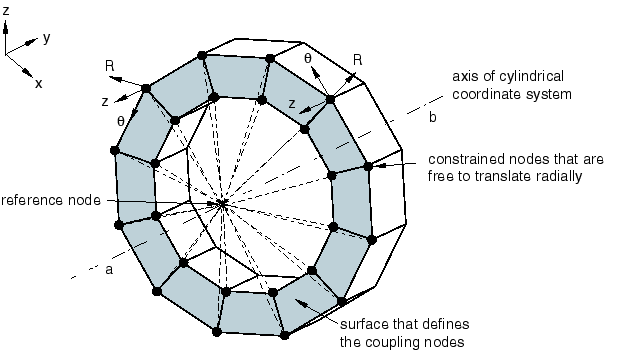
\includegraphics[width=0.8 \textwidth]{model/pcoupling-kinematic}
      \caption[Kinematic coupling constraint]{Kinematic coupling constraint. The sketch illustrates the use of a kinematic coupling constraint to prescribe a twisting motion to a model without constraining the radial motion. In this case, a local cylindrical reference system is used and the constrained nodes have two degrees of freedom coupled to those of the reference node, the angular position $\theta$ and the position along the $z$ axis. The coupling nodes are therefore free to translate radially, varying $R$. \cite{Abaqus}}\label{fig:kinematicCoupling}
    \end{figure}

    For the considered case, the coupling nodes are those mesh nodes located at the faces of the lattice nodes and the master node is the reference point located in the center of the lattice node. In order to achieve the rigid solid behavior, all the degrees of freedom translational and rotational are coupled. In Figure \ref{fig:couplingThroughRF}, an overview of this coupling condition can be viewed.

    \begin{figure}[!htpb]
      \centering
      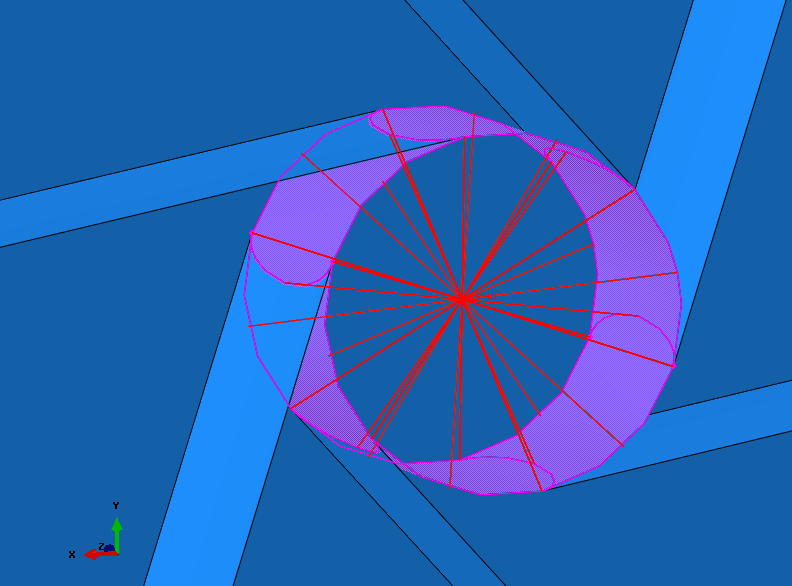
\includegraphics[width=0.6 \textwidth]{model/couplingThroughRF}
      \caption[Overview of the elements that are involved in the coupling condition at the lattice nodes]{Overview of the elements that are involved in the coupling condition at the lattice nodes. The coupling condition was defined in between the mesh nodes located in the faces of the lattice node and a reference point located in the middle. All the degrees of freedom translational and rotational are linked.}\label{fig:couplingThroughRF}
    \end{figure}

    \clearpage
    Another approach consisted in embedding an additional part inside the lattice nodes to add rigidity to the element. The proposed design of such a part, which is referred as tyre from now on, can be seen in Figure \ref{fig:tyre-part}. The internal dimensions of this element are shown in Figure \ref{fig:tyre-internalParameters}. Its dimensions are dependent on parameters of the chiral lattice, that is, the thickness of the tyre is equal to that of the chiral lattice $r_{\mathrm{tyre}} = r_{\mathrm{chi}}$ and the same occurred for the height $B_{\mathrm{tyre}}$ and the radius $r_{\mathrm{tyre}}$ which were $r_{\mathrm{tyre}} = r_{\mathrm{chi}}$ and $B_{\mathrm{tyre}} = B_{\mathrm{chi}}$. The added rigidity was obtained as a result of considering a different material for the tyre such that the Young's modulus of the two parts verify the condition $E_{\mathrm{tyre}} \gg E_{\mathrm{chi}}$. Once, the connection is completed, the resulting merged part looked as shown in Figure \ref{fig:tyre-connection}.

    \begin{figure}[!htpb]
      \centering
      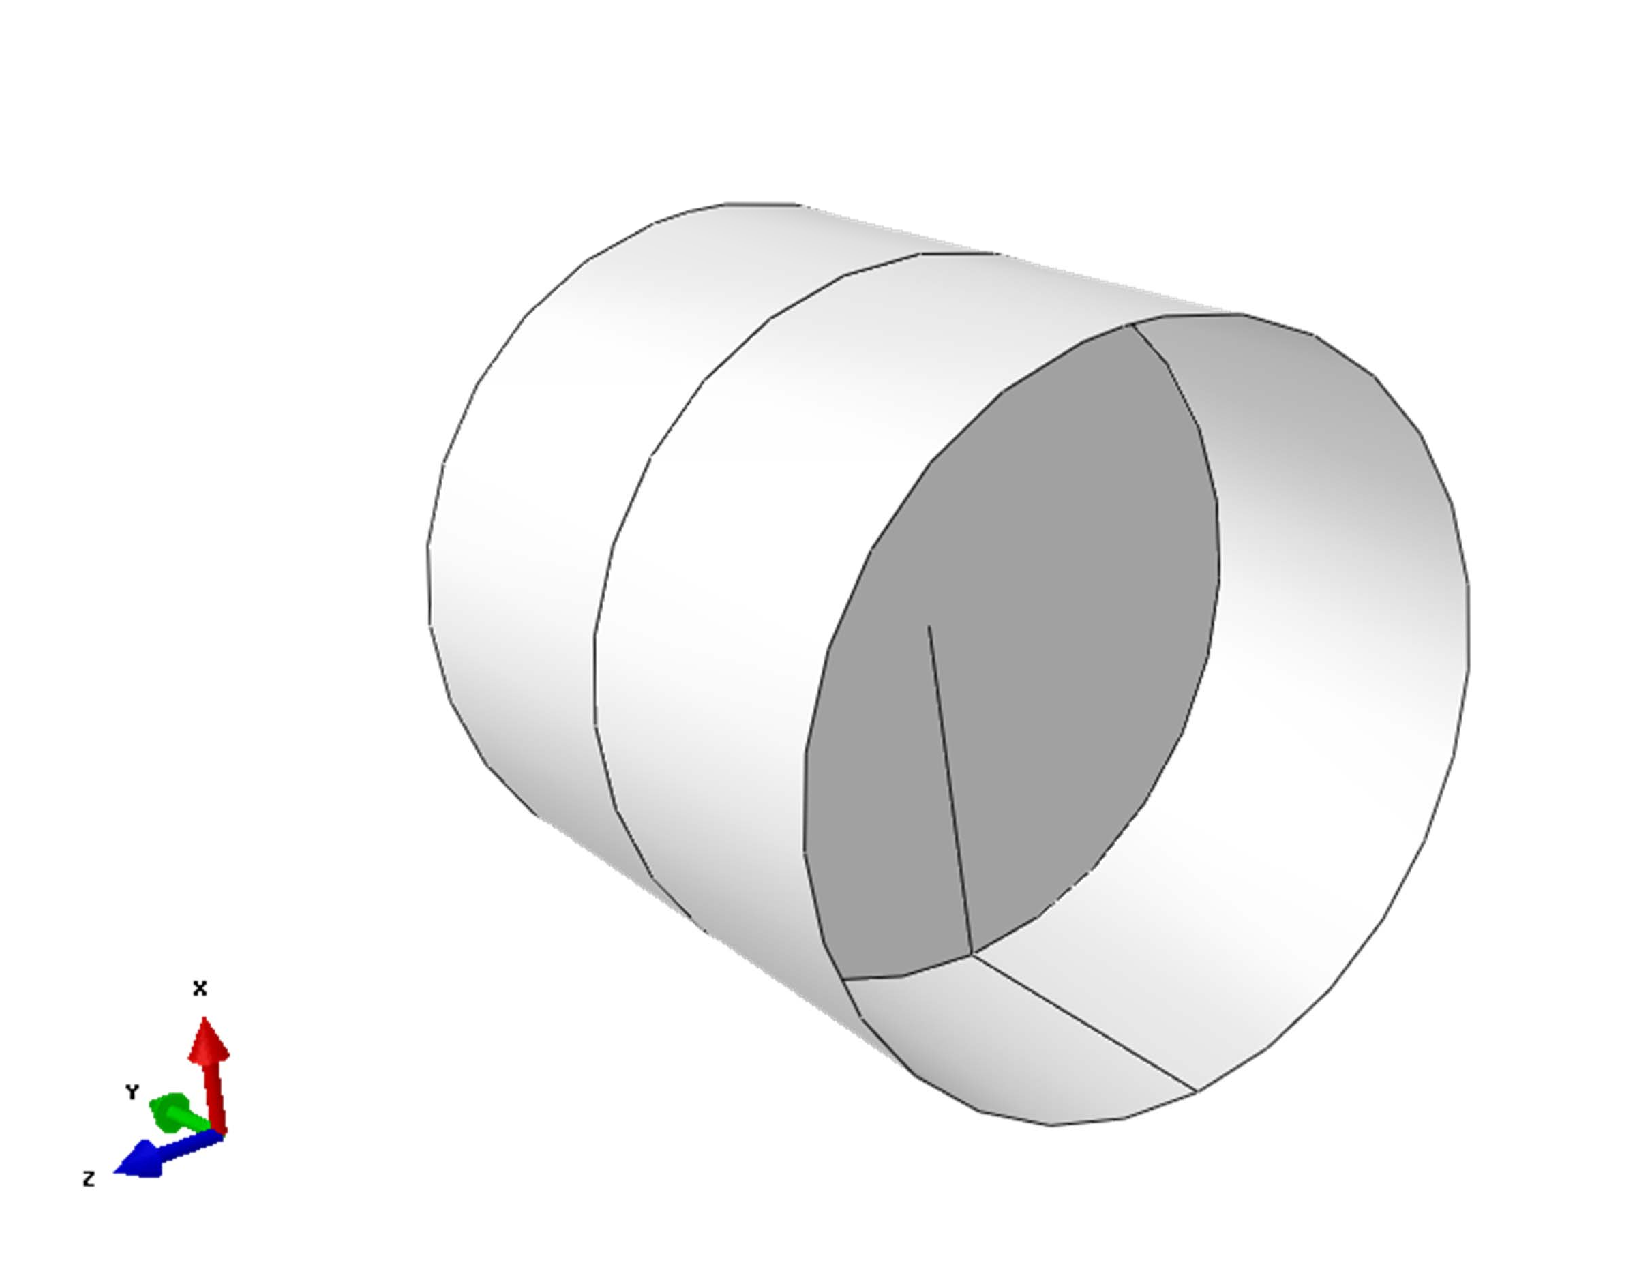
\includegraphics[width=0.6 \textwidth]{model/tyre-part}
      \caption[Overview of the tyre part]{Overview of the tyre part.}\label{fig:tyre-part}
    \end{figure}

    \begin{figure}[!htpb]
      \centering
      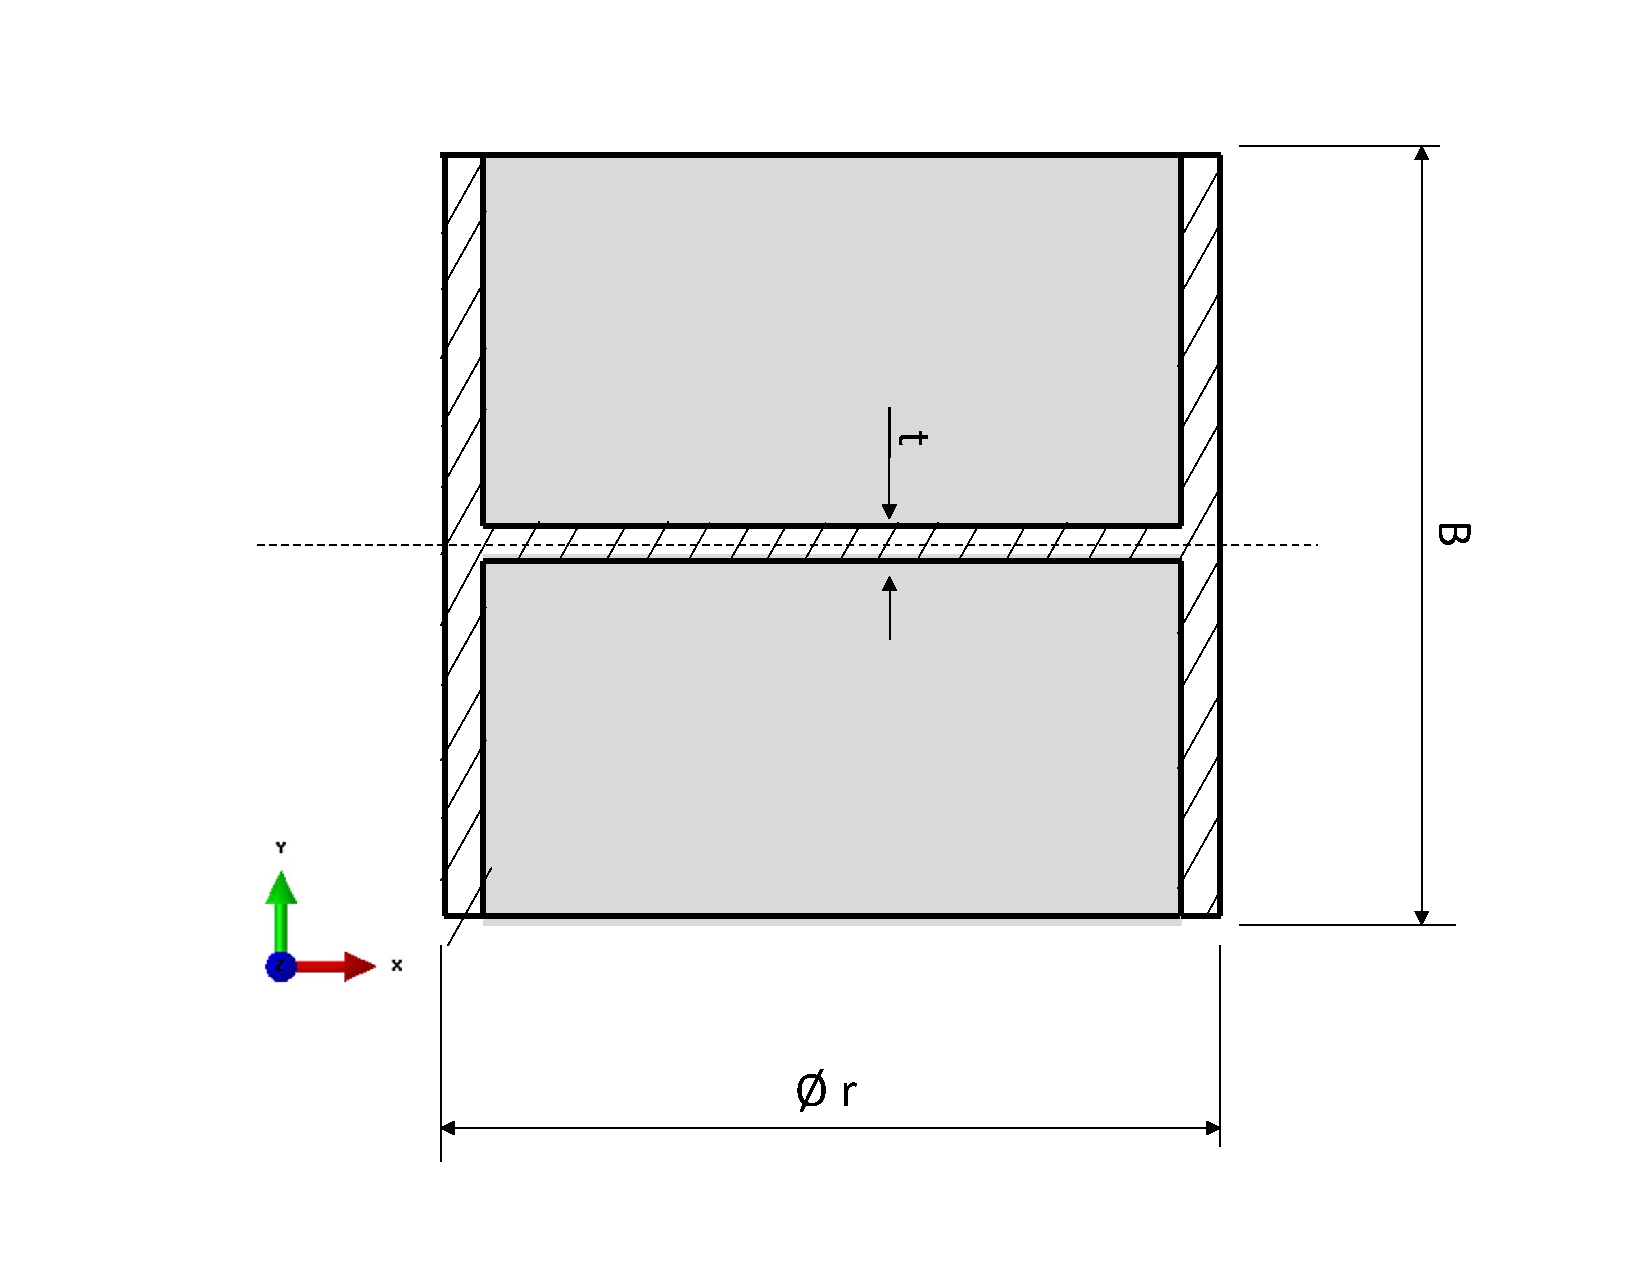
\includegraphics[width=0.8 \textwidth]{model/tyre-internalParameters}
      \caption[Internal parameters of the tyre part]{Internal parameters of the tyre part. The sketch shows a transversal cut to the part. The tyre is characterized by the radius $r_{\mathrm{tyre}}$, the height $B_{\mathrm{tyre}}$ and the thickness $t_{\mathrm{tyre}}$. All this parameters are set to be equal to the corresponding ones in the lattice nodes, therefore: $r_{\mathrm{tyre}} = r_{\mathrm{chi}}$, $B_{\mathrm{tyre}} = B_{\mathrm{chi}}$ and $t_{\mathrm{tyre}} = t_{\mathrm{chi}}$.}\label{fig:tyre-internalParameters}
    \end{figure}

    \begin{figure}[!htpb]
      \centering
      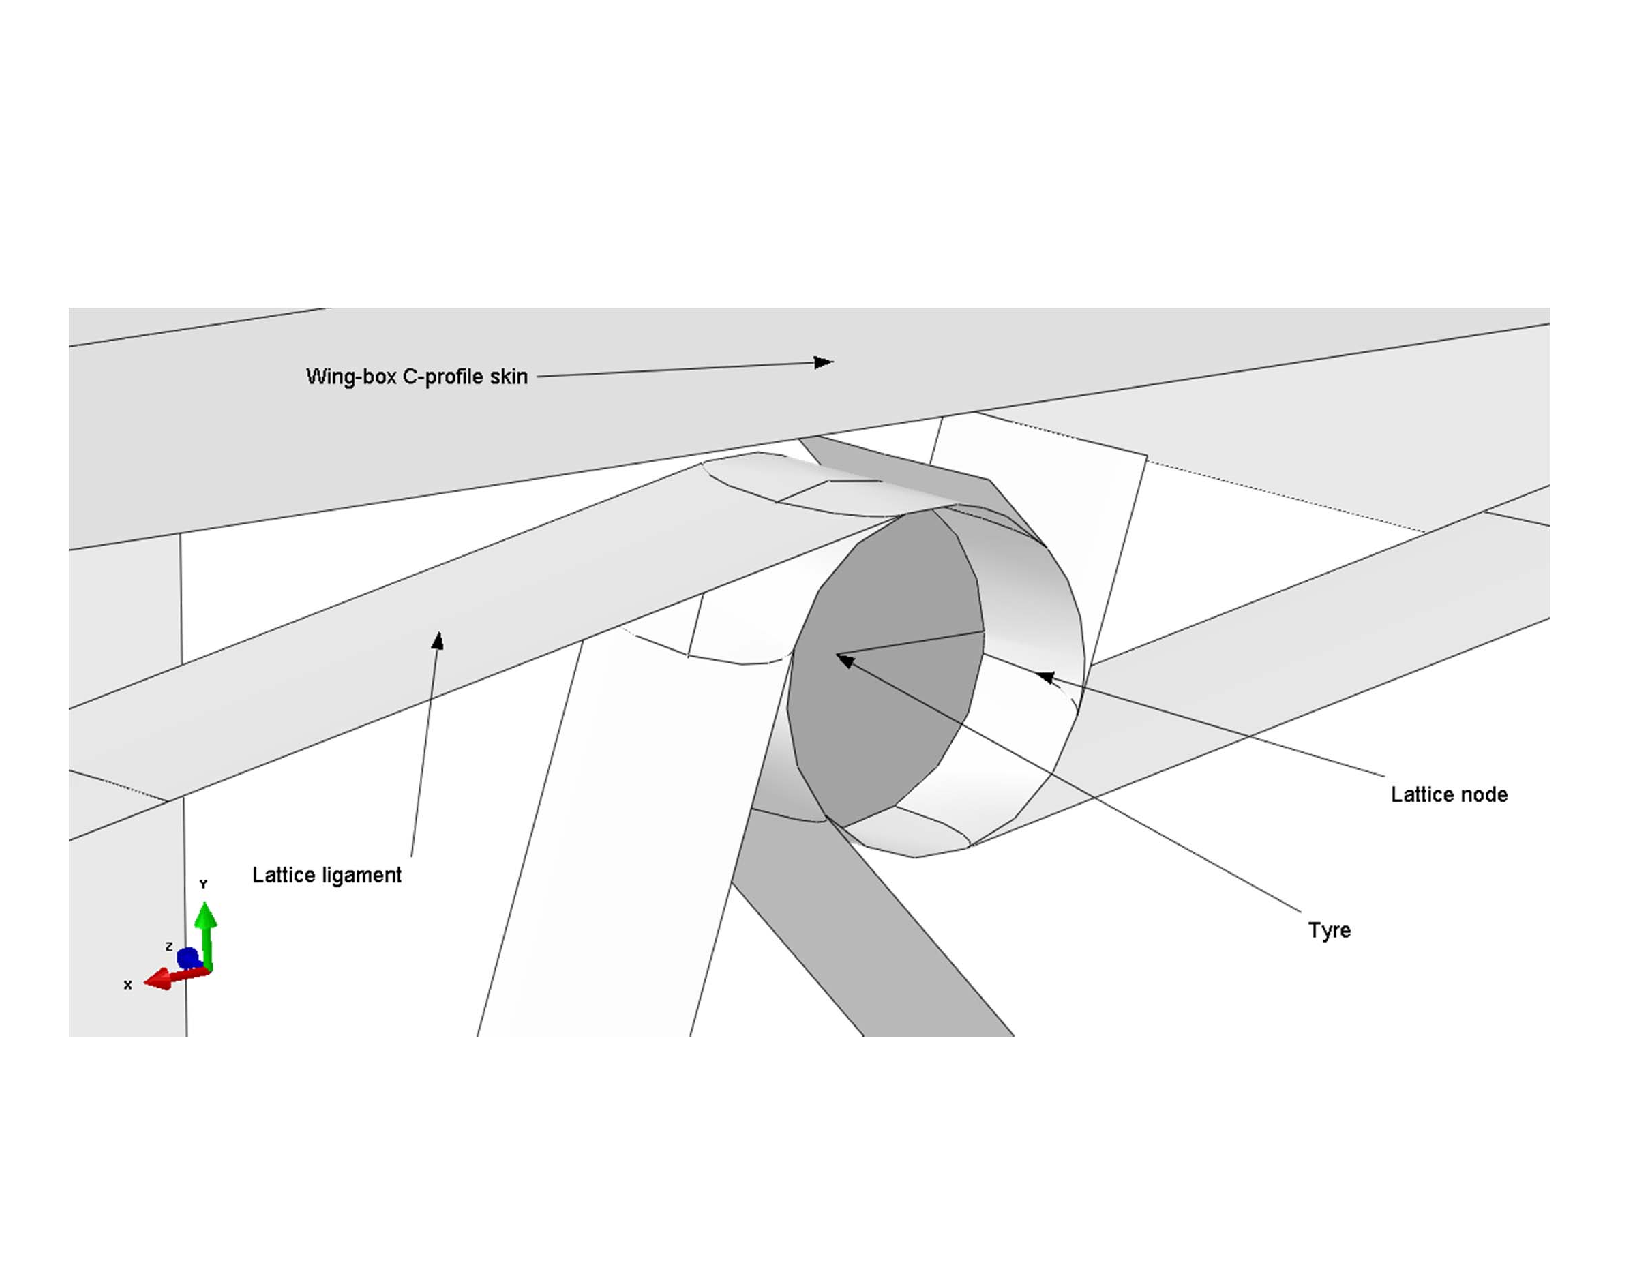
\includegraphics[width=0.8 \textwidth]{model/tyre-connection}
      \caption[Overview of the connection between tyre and lattice node]{Overview of the connection between tyre and lattice node. The tyre will be embed inside the lattice node.}\label{fig:tyre-connection}
    \end{figure}

  \clearpage
  \subsection{Computational model mesh characteristics} \label{subsec:mesh_computationalModel}

    In the present section, the characteristics of the model spatial discretization are presented. The mesh is unstructured and it is auto-generated by Abaqus CAE for the whole assembly. The elements are a combination of quadratic and tetrahedral with 4 and 3 nodes, respectively. Different mesh elements size are assigned to different parts of the model depending of the geometrical complexity of the area.

    In Figure \ref{fig:mesh}, it is possible to distinguish the two regions that are assigned with different mesh element size: the lattice of chiral structures and the close region of the wing-box skin are assigned with a fine mesh size while the remaining model is assigned with a course mesh size, typically one order of magnitude greater. This introduces two new parameters that are used to modify the mesh size of the different regions:
    %
    \begin{itemize}
      \item $S_{\mathrm{f}}$: Fine mesh size, typically equal to 3 mm.
      \item $S_{\mathrm{c}}$: Course mesh size, typically equal to 30 mm
    \end{itemize}

    The selection of this typical values for $S_{\mathrm{f}}$ and $S_{\mathrm{c}}$ are obtained after a number of trial-error attempts to achieve convergence in the nonlinear simulations. As part of the program built to execute the nonlinear simulations, the mesh size is automatically changed if convergence is now achieve. The methodology followed by this program is explained in detail in Subsection \ref{subsec:parametricStudy_computationalModel}.

    \begin{figure}[!htpb]
      \centering
      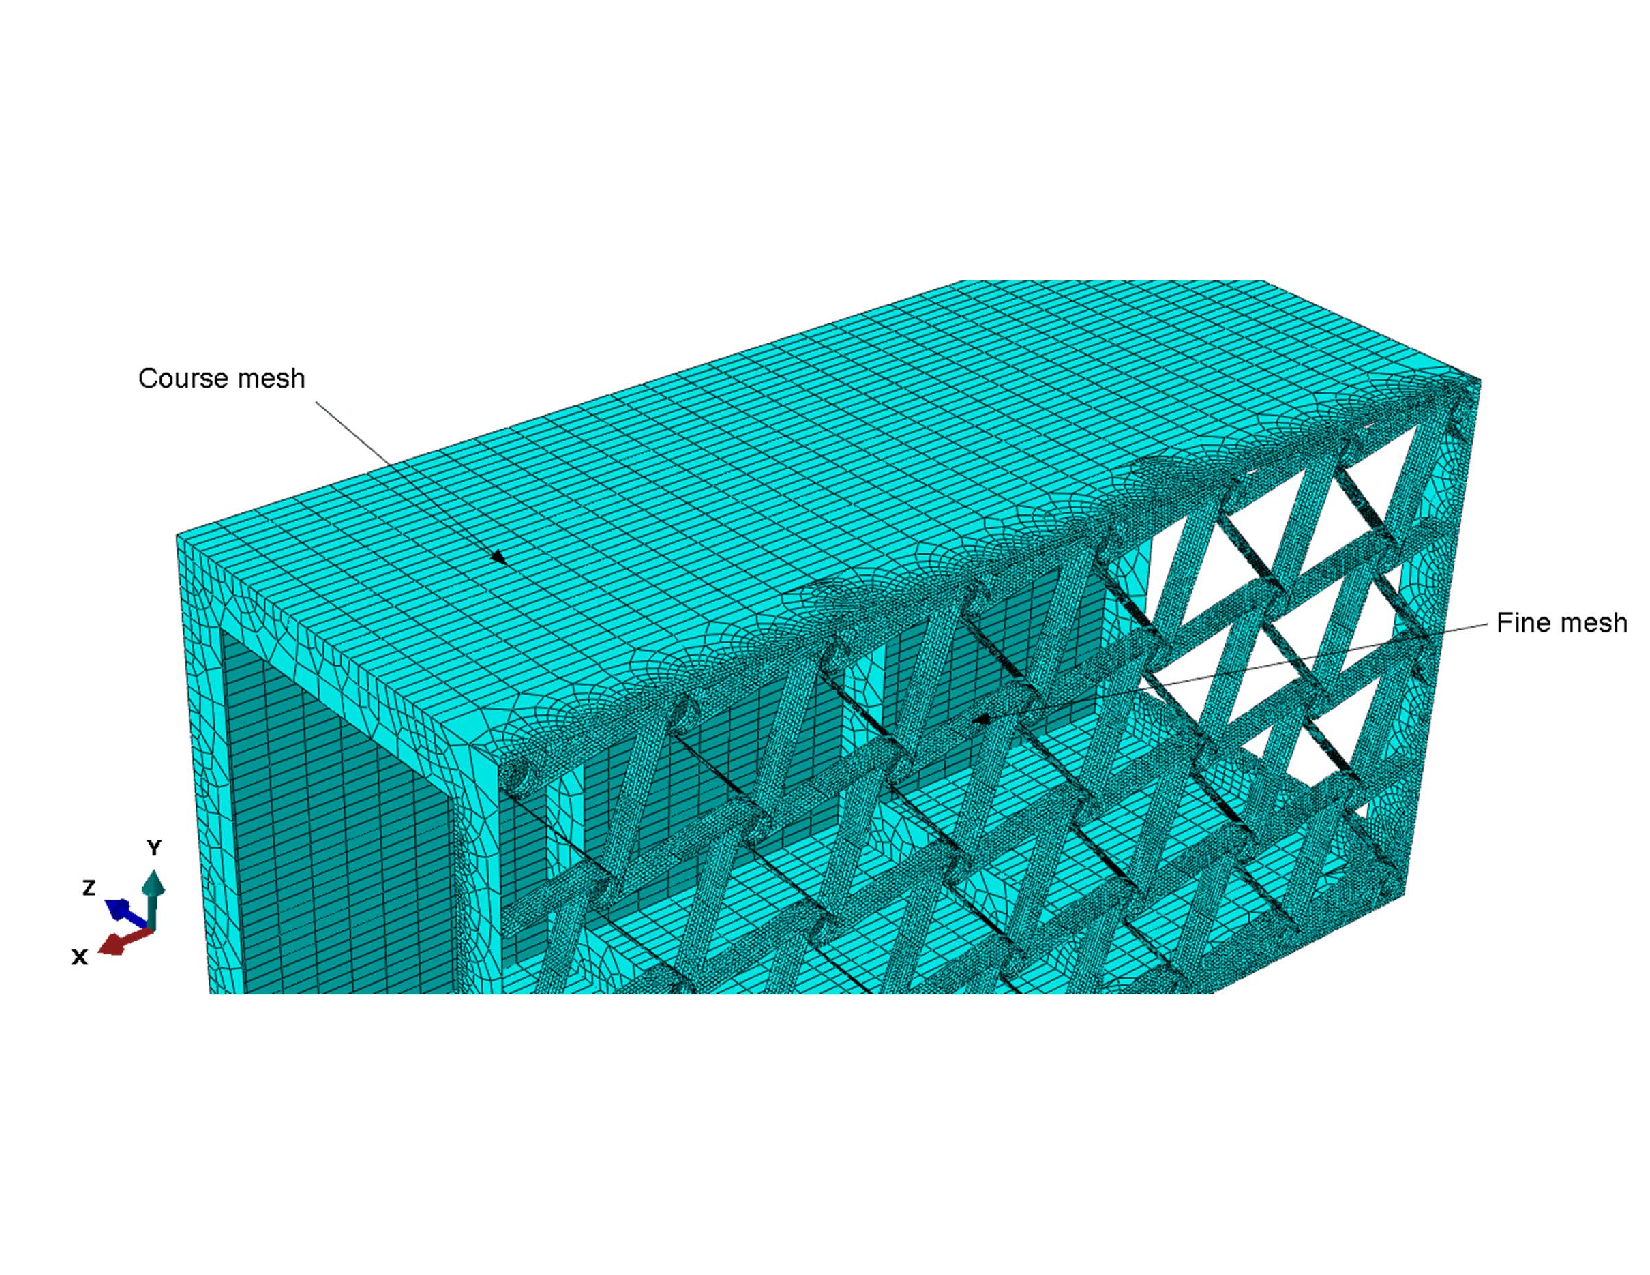
\includegraphics[width=0.8 \textwidth]{model/mesh}
      \caption[Internal parameters of the two different ribs parts]{Internal parameters of the two different ribs parts. Different mesh element size are assigned to different parts of the model. The lattice structure is assigned with a fine mesh element size while the wing-box is assigned with a course mesh element size.}\label{fig:mesh}
    \end{figure}

  \clearpage
  \subsection{Load definition} \label{subsec:load_computationalModel}

    The computational model allowed different possibilities in terms of the load introduction. Among all of them, it was decided to locate the load introduction points on the upper flange of the ribs. The reason for this is the replicate how the load will be introduced in a future manufactured demonstrator of the wing-box.

    Therefore, the number of load introduction points had an upper bound equal to the number of ribs available. For the baseline configuration, this number equals to three, one close rib at the tip of the wing-box and two open ribs in the inner part of the wing-box. Another possibility is to vary the position in the chordwise direction of load introduction point or points. In Figure \ref{fig:loadIntroductionPoints} it can be seen the location of the load introduction points when they are distributed among the three available ribs and their position in the chordwise direction is equal to $z / = 0.8 $.

    In Subsection \ref{subsec:load_results_model}, the differences in the response of the structure depending on the number of load introduction points that their position in the chordwise direction are discussed.

    \begin{figure}[!htpb]
      \centering
      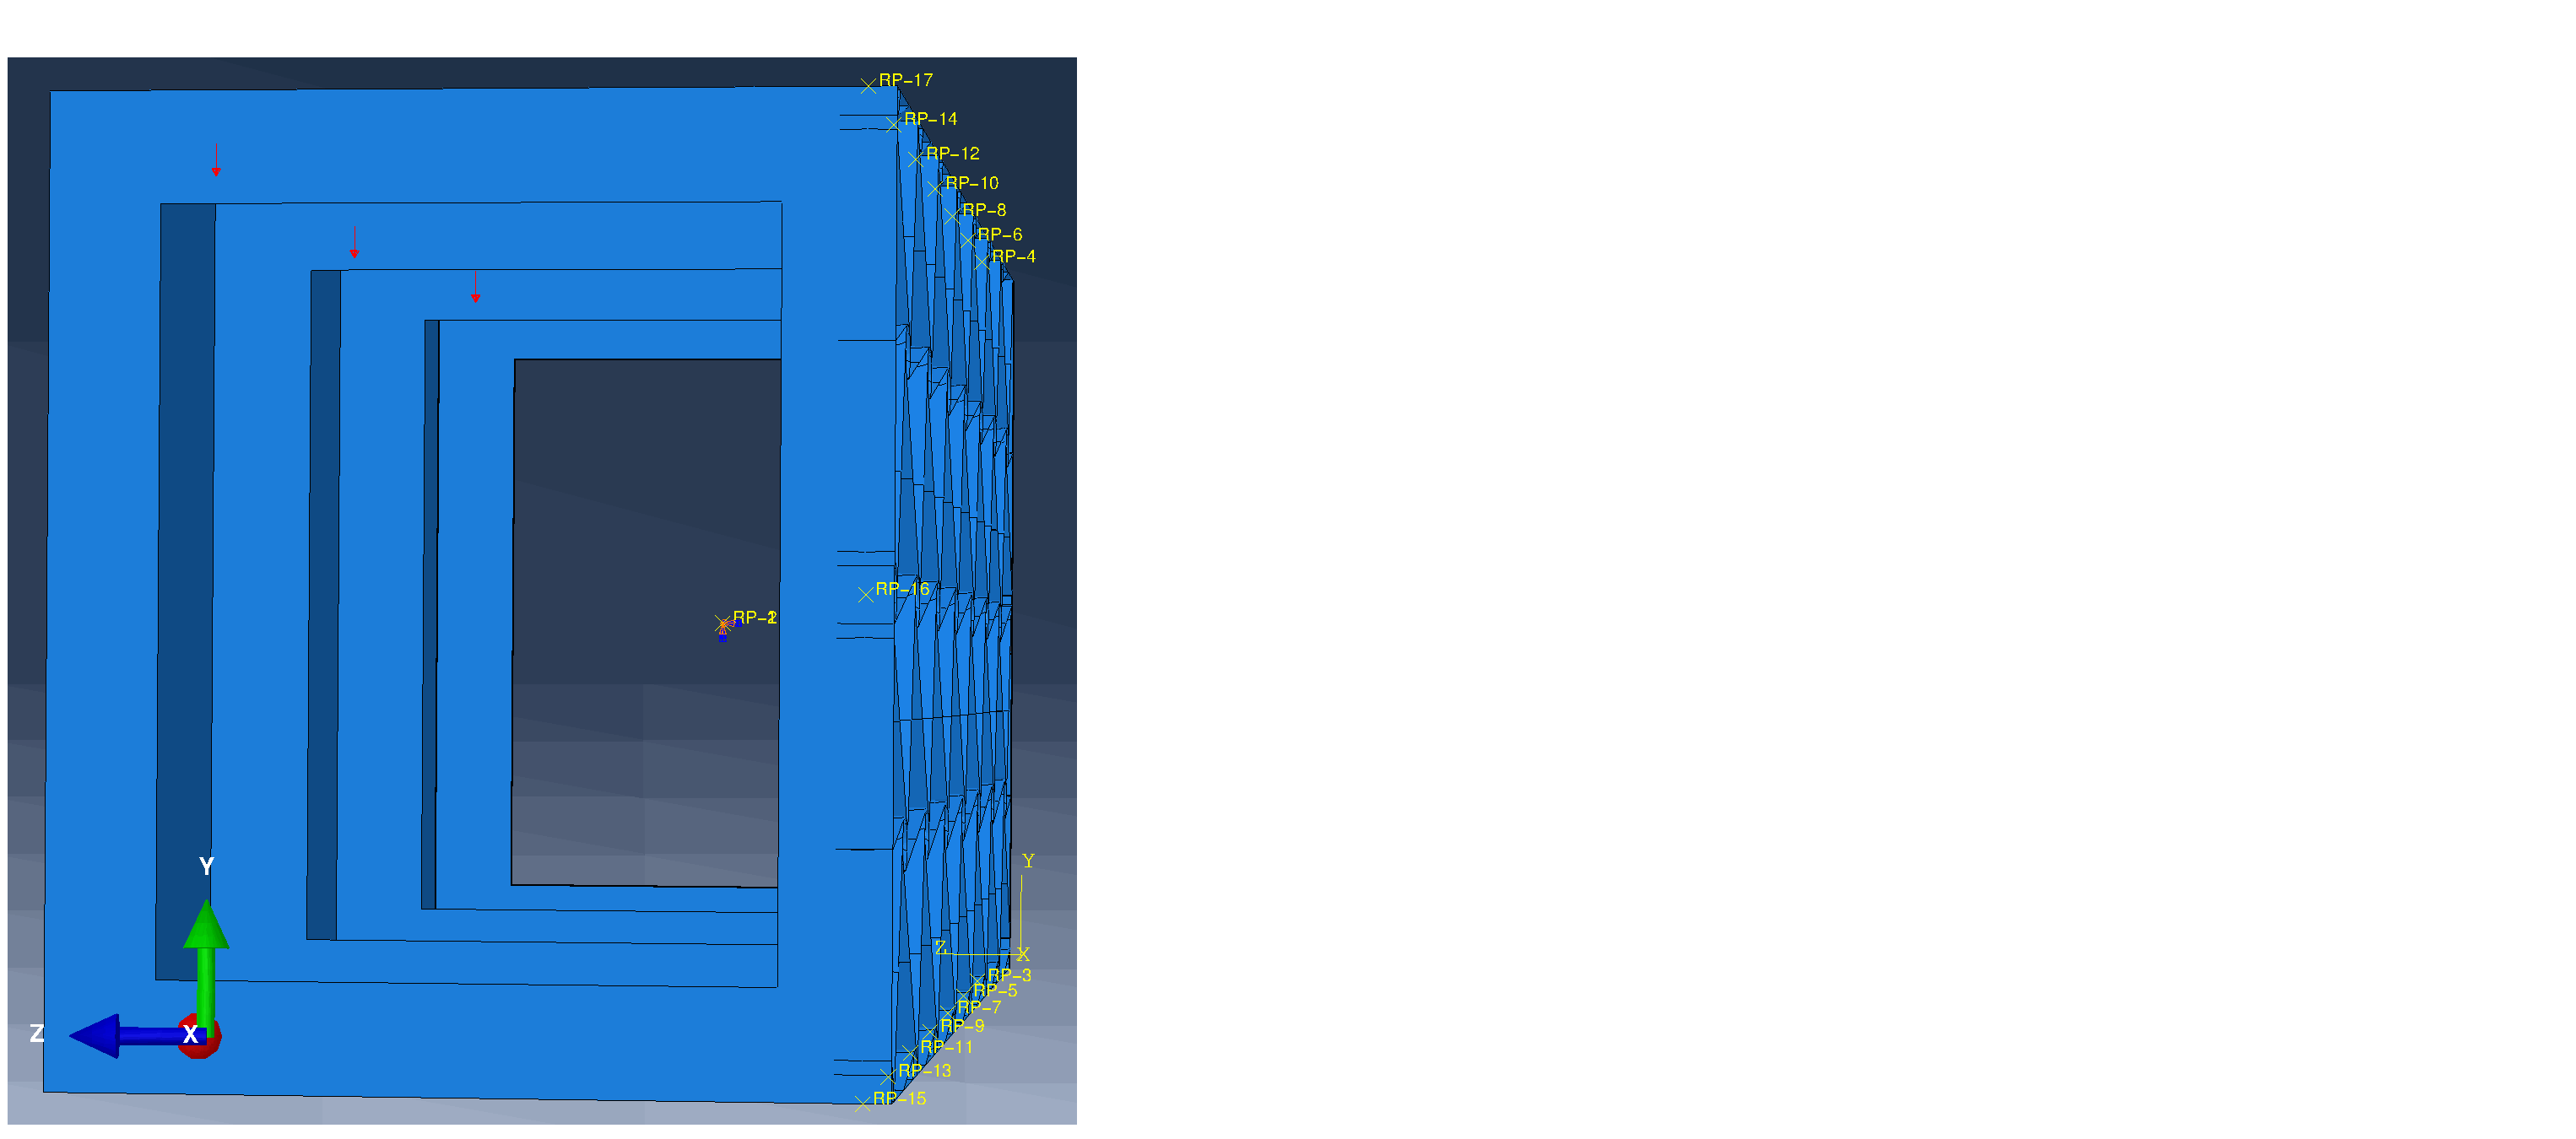
\includegraphics[width=0.6 \textwidth]{../figures/model/loadIntroductionPoints}
      \caption[Load introduction points located on the upper flange of the tip rib and the two inner ribs]{Load introduction points located on the upper flange of the tip rib and the two inner ribs.}
      \label{fig:loadIntroductionPoints}
    \end{figure}

  % \clearpage
  \subsection{Boundary condition} \label{subsec:boundary_computationalModel}

    The boundary condition for the whole assembly is the one shown in Figure \ref{fig:fixed}. It consisted in a kinematic coupling similar to the one introduced in Section \ref{subsec:parametrization_Model} to model the rigid body behavior of the lattice nodes. In this case, the kinematic coupling is establish between a reference point located approximately at the centre of the root rib and the faces of this mentioned rib. The reference point acts as a master node while the mesh nodes located at the faces of the rib are the slave nodes. The reference point is next fixed in all its degrees of freedom using the corresponding boundary condition Abaqus module.

    \begin{figure}[!htpb]
      \centering
      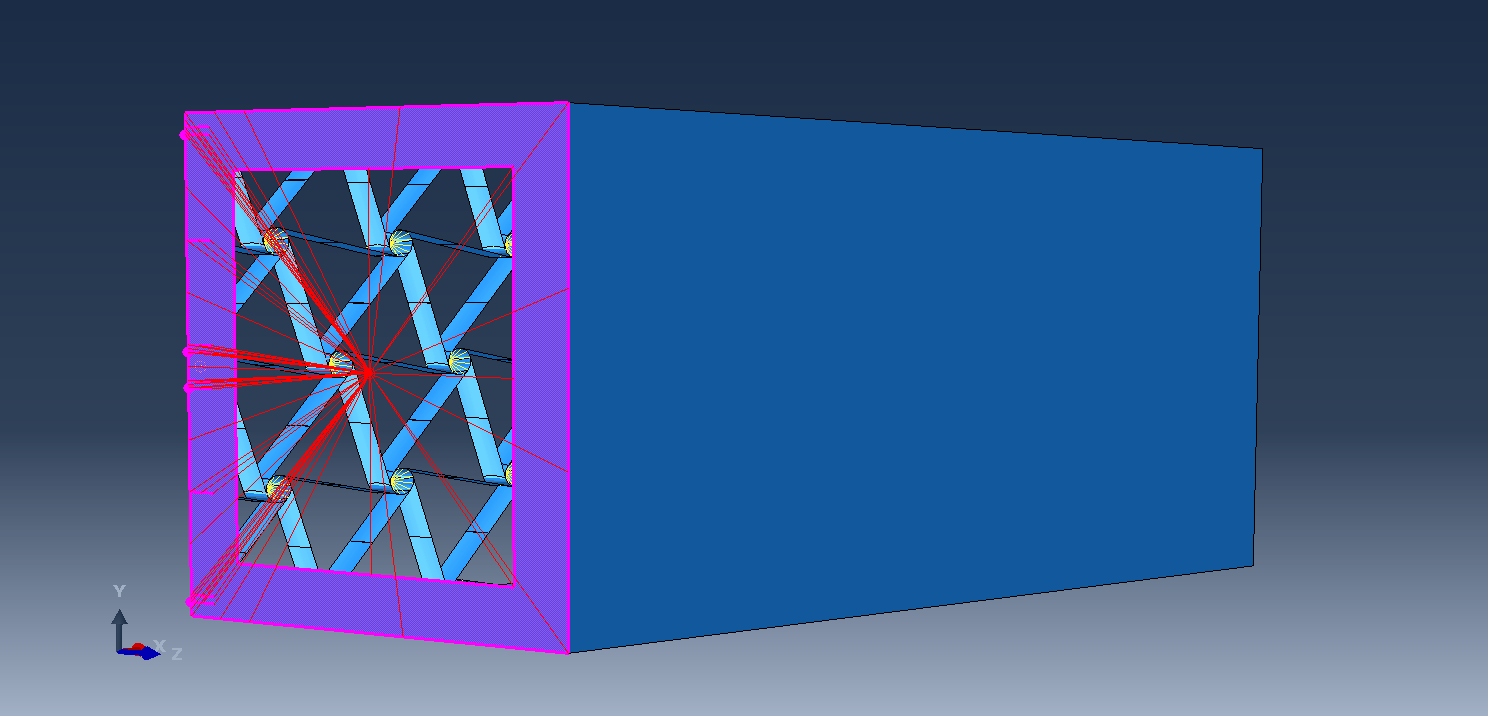
\includegraphics[width=0.8 \textwidth]{../figures/result-model/fixed}
      \caption[Boundary condition for the model]{Boundary condition for the model. The condition is establish through a coupling interaction between a reference point and the faces of the rib at the root. The reference point is fixed in all its degrees of freedom using the corresponding boundary condition Abaqus module.}\label{fig:fixed}
    \end{figure}

  % \clearpage
  \subsection{Post-processing operations} \label{subsec:postProc_computationalModel} %To be extended, maybe

    The results obtained from the Abaqus simulations were analysed in two different ways. Firstly, qualitatively by means of the deformation plots that shown the corresponding Abaqus visualization module. And, secondly, extracting values of different magnitudes directly from the mesh nodes or elements located at certain positions of interest on the solution model.

    Through the definition of paths in Abaqus, it is possible to obtain the value of a determined magnitude for all the mesh elements located along the path. In Figure \ref{fig:pathUpper}, an example of a path located on the upper skin of the wing-box is shown.

    In the Python program written to run the parametric analysis, a special module is executed to extract information from the the Abaqus solution model. This piece code is able to extract magnitude values from different parts of the model, using paths. In the case of the rotational displacement $u$ around the $x$ direction, the value of the corresponding magnitude is extracted from mesh elements on the upper and lower flange of the wing-box, and also from differences in the displacement $v$ along the transversal direction $y$. The final value of the rotation is obtained calculating the mean of the previous values. The error in this calculation is also included in the tables that contain results from the simulations.

    \begin{figure}[!htpb]
      \centering
      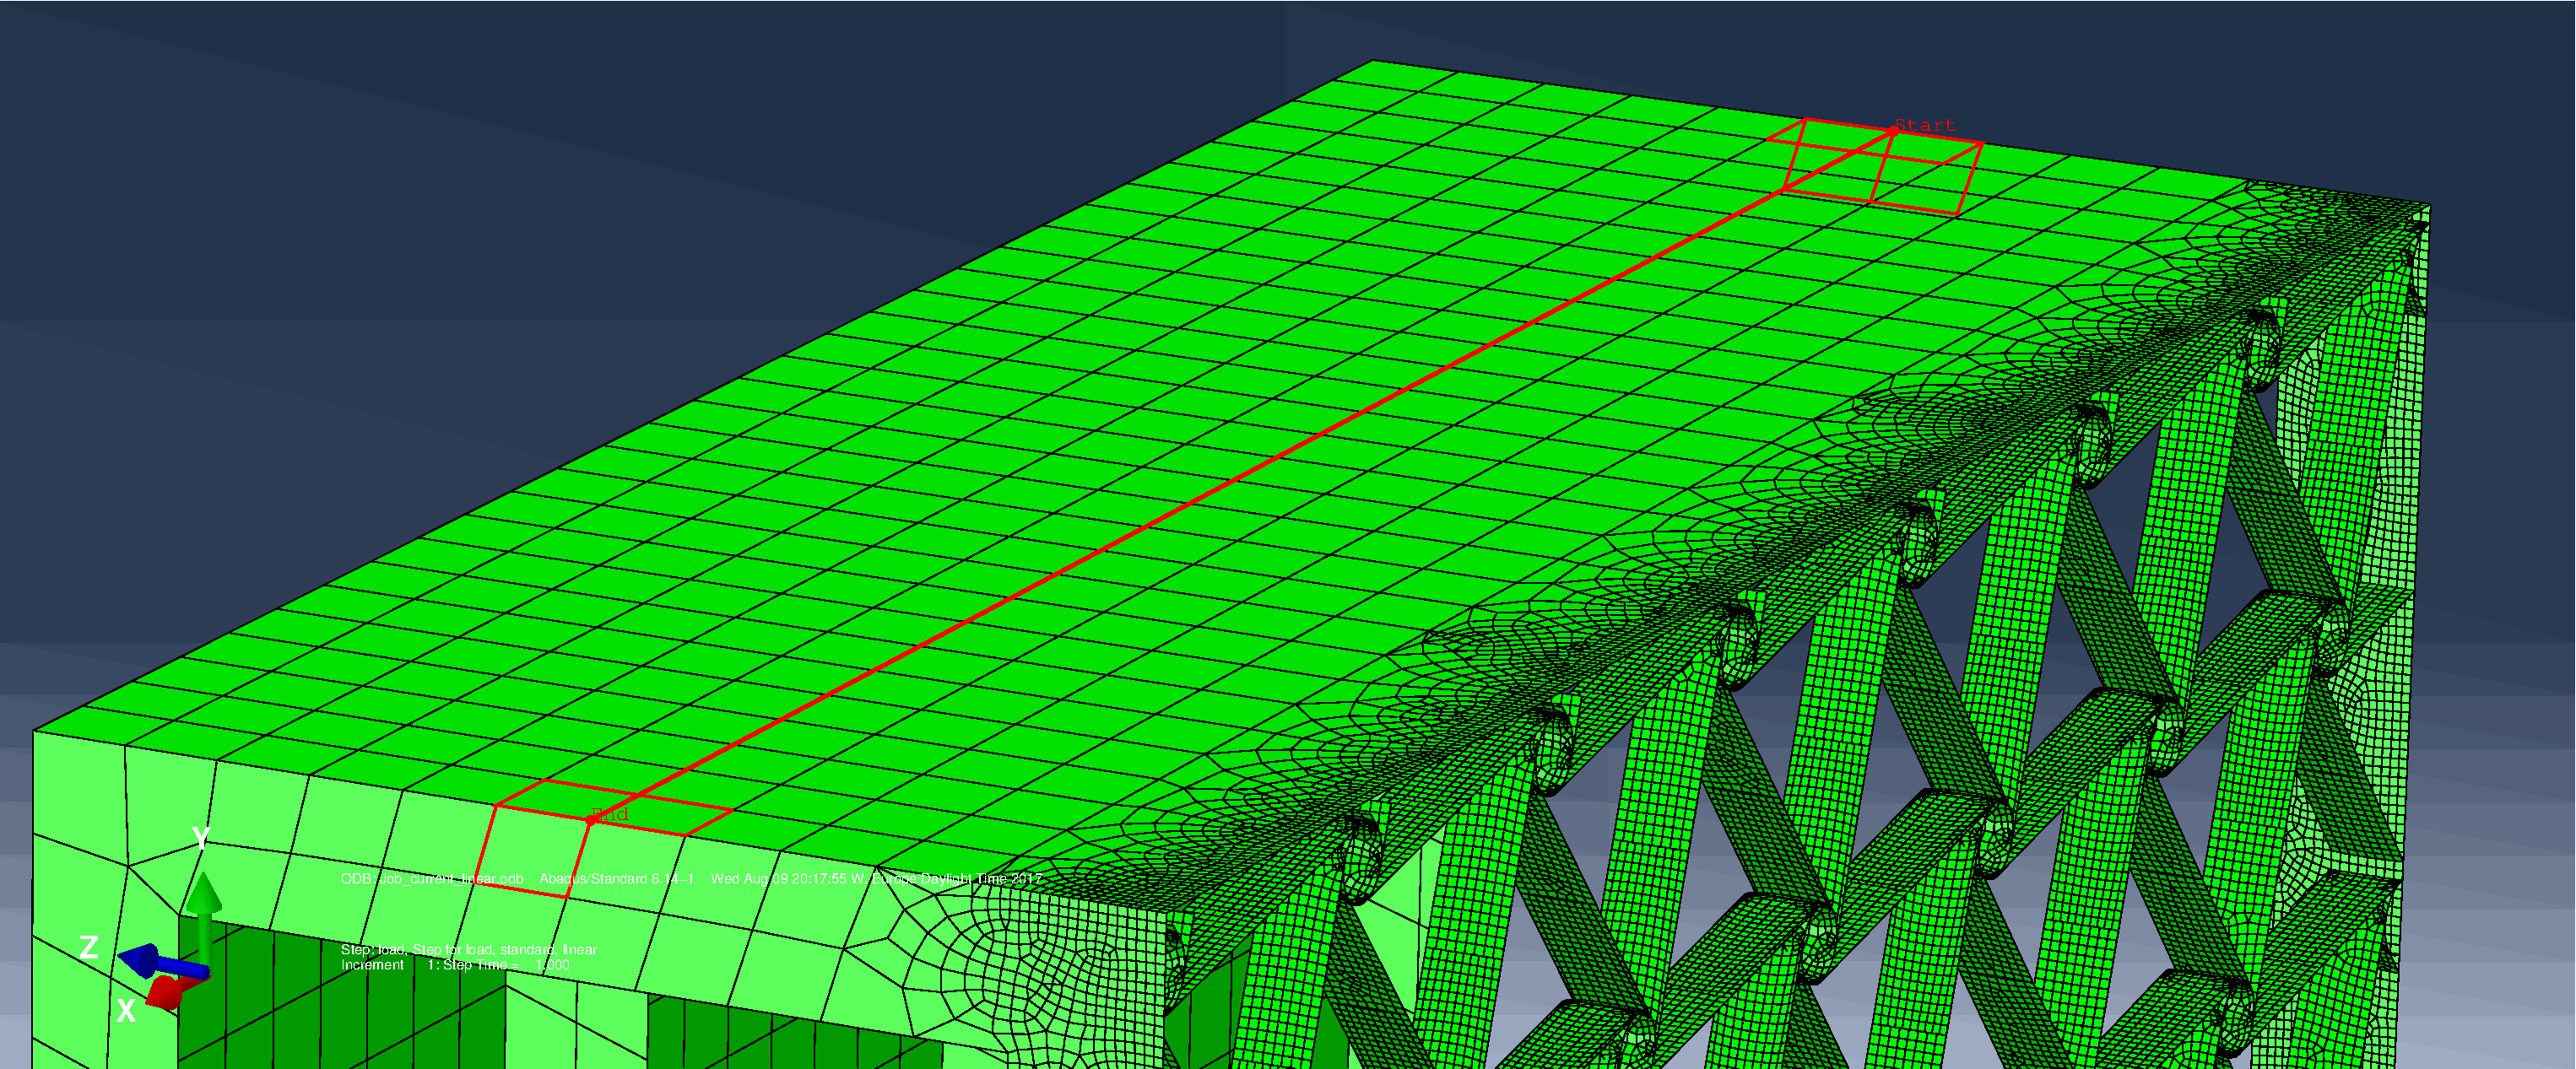
\includegraphics[width=0.8 \textwidth]{../figures/result-model/pathUpper}
      \caption[Path of mesh elements on the solution model]{Path of mesh elements on the solution model.}\label{fig:pathUpper}
    \end{figure}
  
  \clearpage
  \subsection{Parametric study method} \label{subsec:parametricStudy_computationalModel}

    The model described in the previous subsections is implemented in a Python program that is read by the FEM software, Abaqus CAE. The program is fully parametrized and this enables the possibility of executing simulations for different values of the parameters introduced previously. The parametric study program is executed when calling the python file \texttt{mainAbaqusParametricStudy.py}. As part of the execution of this file, a computational model is built, submitted for analysis and post-processed by the complementary program \texttt{mainBuildAndExecuteWingBox.py}, for all the different values of the parameters that belong to the parametric study defined in the file \texttt{setUpParametricStudy.py}. The convergence of the simulation is controlled within the program \texttt{mainAbaqusParametricStudy.py} and it is able to re-run a simulation with slight variations in the mesh size and/or in artificial dissipation definition if convergence was not achieved.

    An schematic characterization of the program execution is shown the flow chart represented in Figure \ref{fig:flowChart}. The code written for this program can be found in Appendix \ref{appen:code}. 

    \begin{figure}[!htpb]
      \centering
      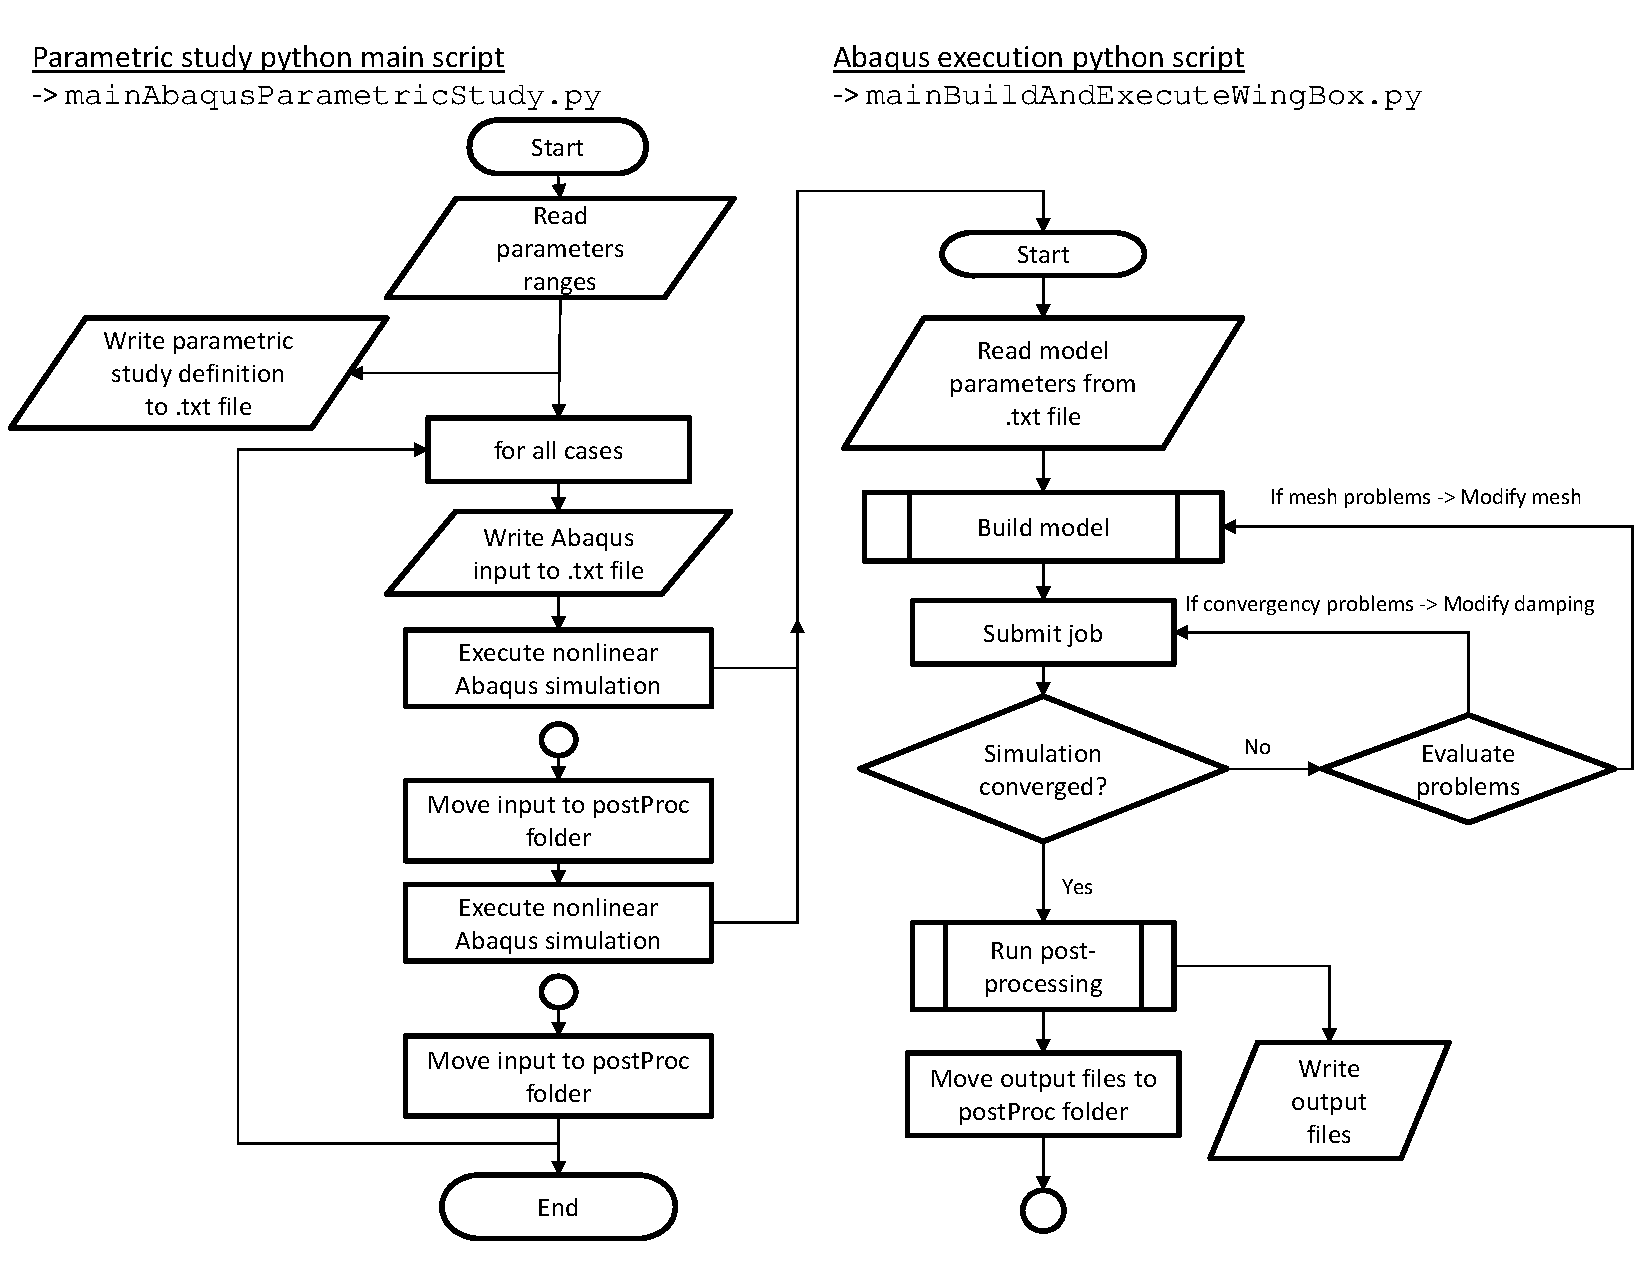
\includegraphics[width=1.0 \textwidth]{model/flowChart}
      \caption[Flow chart showing the execution of the parametric study code]{Flow chart showing the execution of the parametric study python code.}\label{fig:flowChart}
    \end{figure}

  % \clearpage
  % \subsection{Connection between the wing-box skin and the chiral lattice} \label{subsec:connections_computationalModel}

  %   %General thoughts:
  %   % - Necessity of applying condition node to node
  %   %
  %   %Equation contrainsts issues:
  %   % - Slow down simulations
  %   %
  %   %Coupling constrainsts:
  %   %
  %   %
  %   In the present subsection, the computational modeling of the connection between the lattice nodes and the wing-box skin is presented. This is an unavoidable transition from the lattice of chiral structures comprised of nodes and ligaments to the skin of the wing-box. Loads are transmitted to the lattice through this attachment points that is why its design results crucial. Three different configurations are studied:

  %   \begin{description}
  %     \item[Blocked translation and rotation] The lattice nodes have all its degrees of freedom restrained 
  %     \item[Blocked translation and free rotation] The lattice nodes are only restraint in the rotation around its own axis by the ligaments. The translation displacement parallel to the skin is restrained. An sketch showing this connection can be viewed in Figure \ref{fig:connectionModeling1}. This configuration was the one chosen for the demonstrator built in the Figure \ref{fig:connectionLatticeNodesToSkin}.
  %     \item[Free translation and rotation] Now the lattice nodes are also allowed to translate parallel to the skin. This configuration is schematically represented in Figure \ref{fig:connectionModeling2}.
  %   \end{description}

  %   \begin{figure}[!htpb]
  %     \centering
  %     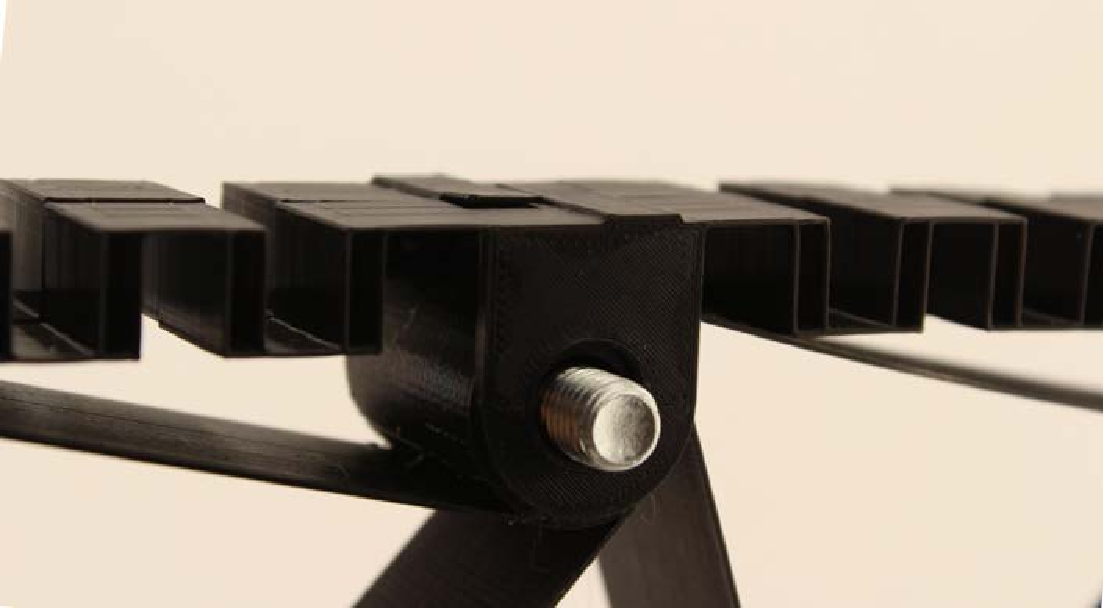
\includegraphics[width=0.8 \textwidth]{model/connectionLatticeNodesToSkin}
  %     \caption[Detail of the connection between the lattice nodes and the skin]{Detail of the connection between the lattice nodes and the skin. The picture shows the type of connection chosen for the manufactured demonstrator of the lattice. The lattice nodes is allowed to rotate around its own axis but cannot translate parallel to the skin. This photography was taken from the demonstrator built by \cite{Vincenz2017}.}\label{fig:connectionLatticeNodesToSkin}
  %   \end{figure}

  %   \begin{figure}[!htpb]
  %     \centering
  %     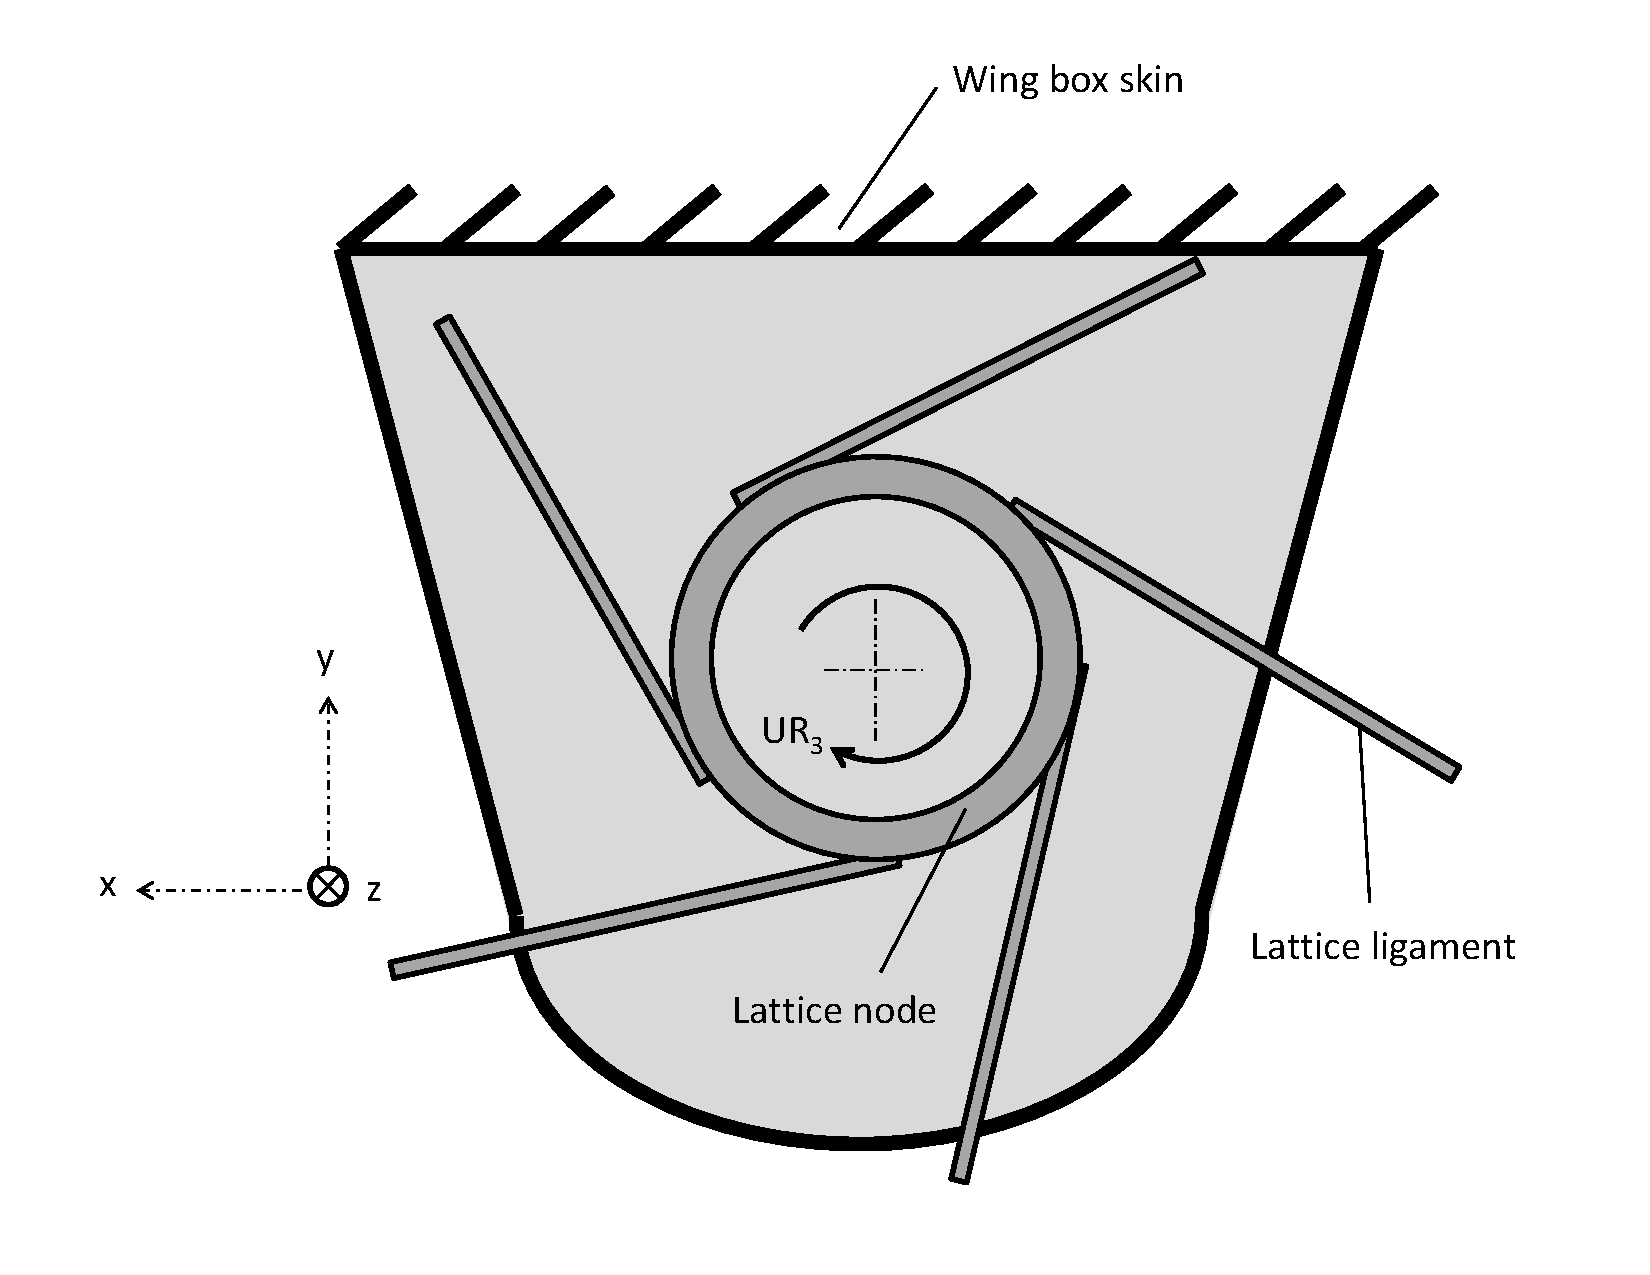
\includegraphics[width=0.6 \textwidth]{model/connectionModeling1}
  %     \caption[Blocked translation and free rotation connection between the lattice nodes and the skin]{Blocked translation and free rotation connection between the lattice nodes and the skin. In this case, the only degree of freedom of the lattice node that it is not restrained the rotation around its own axis, that is the rotation $UR_3$ around the direction $z$.}\label{fig:connectionModeling1}
  %   \end{figure}

  %   \begin{figure}[!htpb]
  %     \centering
  %     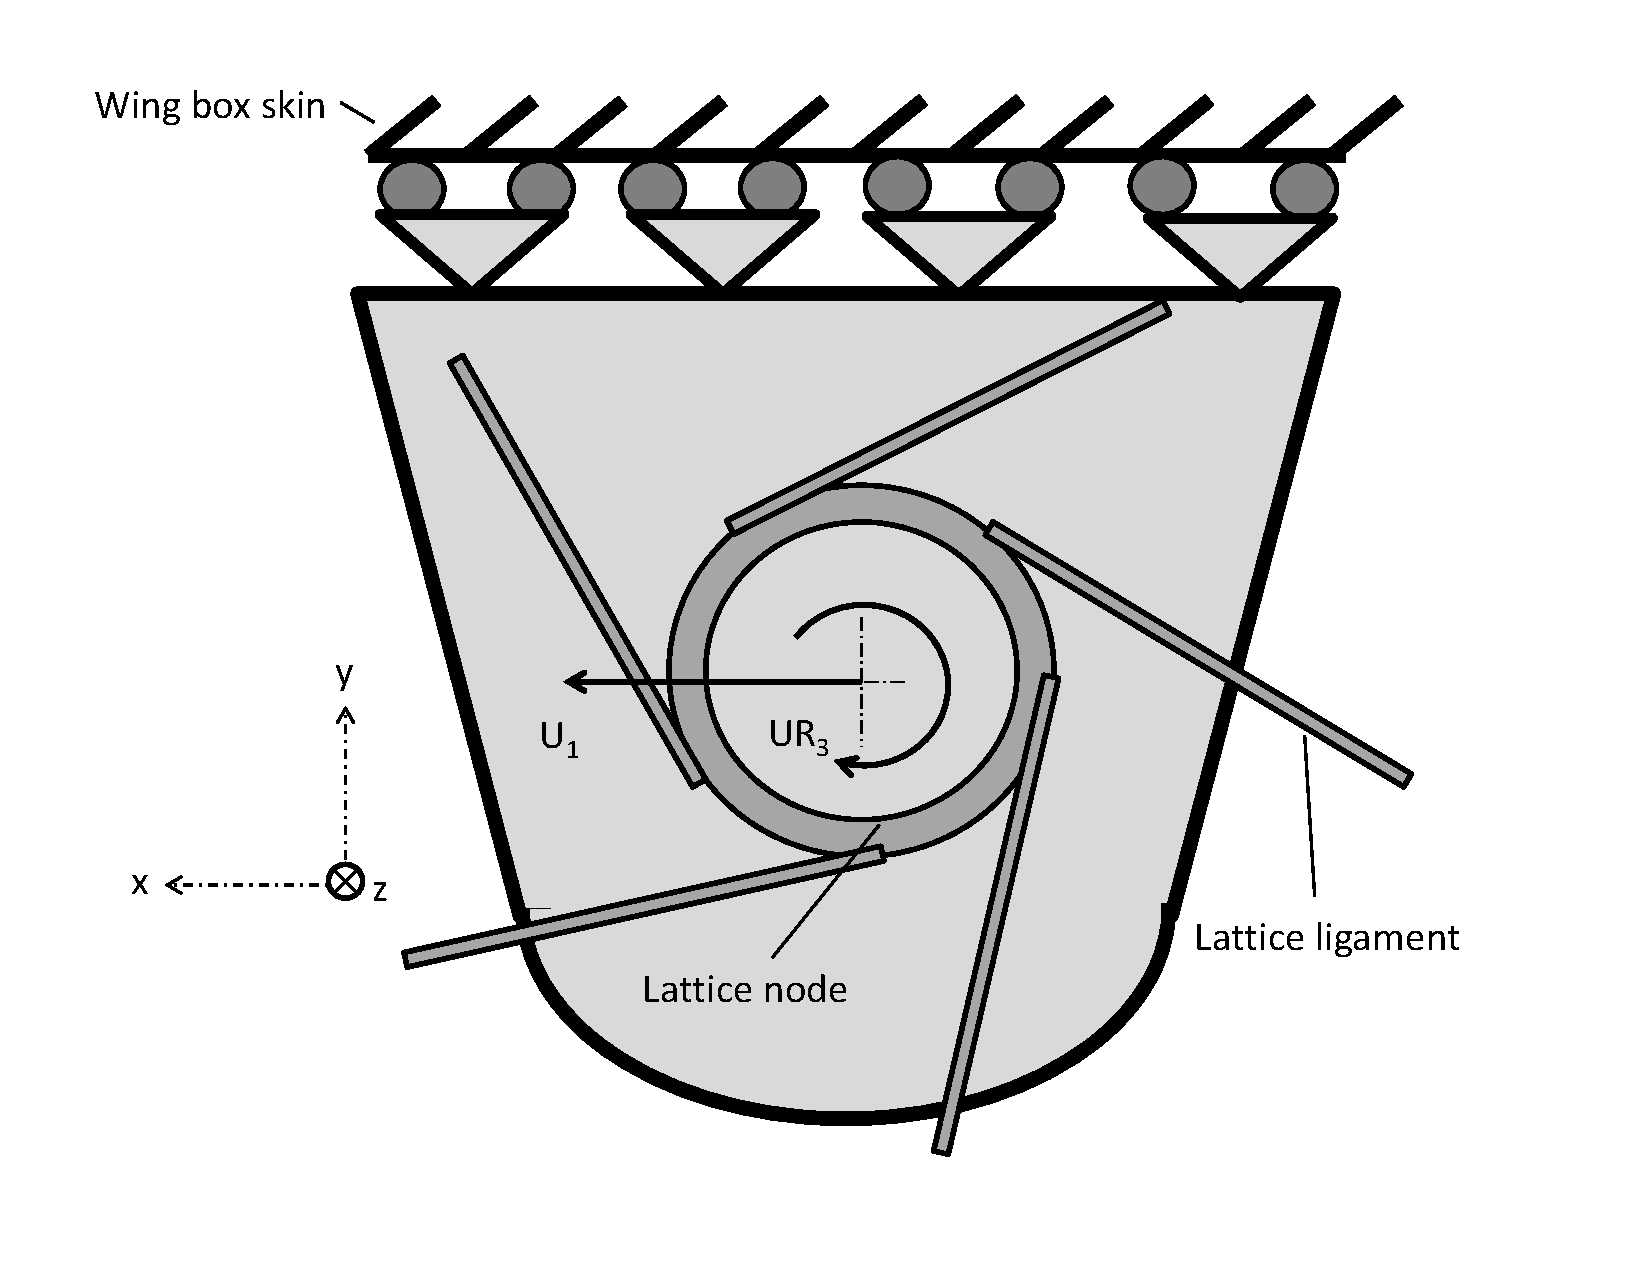
\includegraphics[width=0.6 \textwidth]{model/connectionModeling2}
  %     \caption[Free translation and rotation connection between the lattice nodes and the skin]{Free translation and rotation connection between the lattice nodes and the skin. For this case, the unrestrained degrees of freedom of the lattice nodes are the rotation the rotation $UR_3$ around its own axis, i.e.: the direction $z$; and the displacement $U_1$ parallel to the wing-box wall, i.e.: along the direction $x$.}\label{fig:connectionModeling2}
  %   \end{figure}

  %   In the computational model the lattice of chiral elements and the skin of the wing-box are not physical connected by any element. It becomes necessary to use the interaction module provided by Abaqus CAE to model the connections. Two different approaches are studied to achieve this modeling task. These are presented below.

  %   \subsubsection{Coupling through tyre part}

  %   This approach consists in using the tyre part that was described in Subsection \ref{subsec:parametrization_Model}. At each of the lattice nodes located at the border of the lattice structure, a tyre part is created and embed into the lattice node, as it is shown in Figure \ref{fig:tyre-connection}. Then, a coupling constraint is establish between a mesh node in the middle of the tyre and a mesh node located on the wing-box skin just above the tyre, as shown in Figure \ref{fig:connection-tyre}.

  %   \begin{figure}[!htpb]
  %     \centering
  %     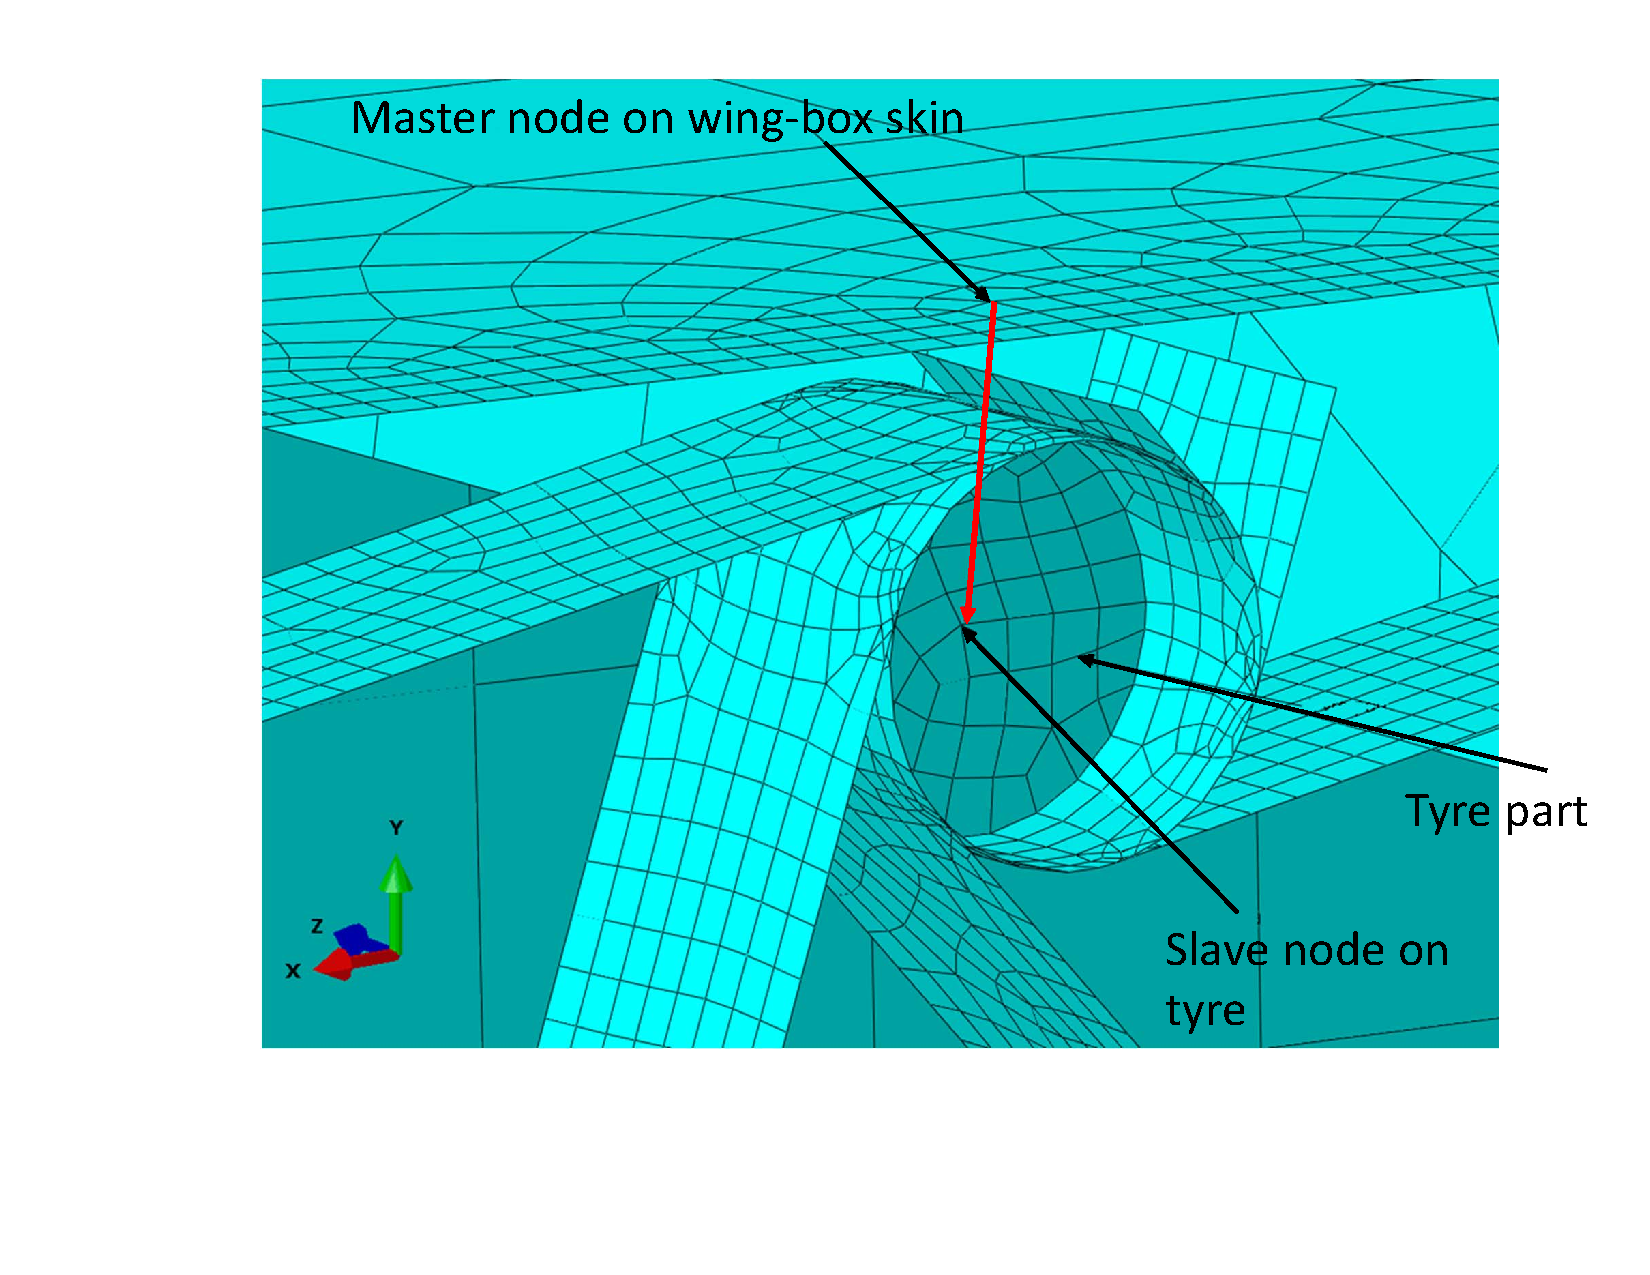
\includegraphics[width=0.8 \textwidth]{model/connection-tyre}
  %     \caption[Coupling condition between the lattice node and the wing-box skin through tyre]{Coupling condition between the lattice node and the wing-box skin through tyre. The coupling condition is establish between a mesh node located in the wing-box skin that acts as a master node and a mesh node in the middle of the tyre that becomes the coupling node.}\label{fig:connection-tyre}
  %   \end{figure}

  %   Depending on the type of connection considered, different degrees of freedom are coupled. For the most restrictive case, in which the connection between the lattice structure and the wing-box is rigid, not allowing any translational or rotational displacement, the six degrees of freedom are coupled between the mesh nodes mentioned on the previous paragraph.

  %   For the other connection types, rotation of the lattice node is allowed around its own axis. This allowance is implemented by not constraining the rotational displacement $w$ around the $z$ direction in the coupling constraint definition. Finally, the last connection type introduced at the beginning of the present subsection allowed the displacement of the lattice node parallel to the wing-box skin. For this case, the translational displacement $u$ along the $x$ direction is be left uncoupled.

  %   The rigid body motion imposed to the mesh node located at the center of the tyre is translated to the mesh nodes located in the faces of the lattice node because they are physically connected.

  %   \subsubsection{Coupling through local cylindrical reference system}

  %   In this case, the rigid body feature provided by the tyre installation is replaced by an additional coupling condition created in a local cylindrical reference system located at each of the lattice nodes. This new reference system substitutes the global Cartesian coordinates system and its origin is a reference point located in the centre of the lattice node,  at $z=B/2$mm. The position of a point in the lattice node face will be determined by the radial distance $r$ to the origin, the angular position $\theta$ and the position $z$ along the lattice node rotation axis. An sketch of this reference system is shown in Figure \ref{fig:connection-localSYS1}.

  %   \begin{figure}[!htpb]
  %     \centering
  %     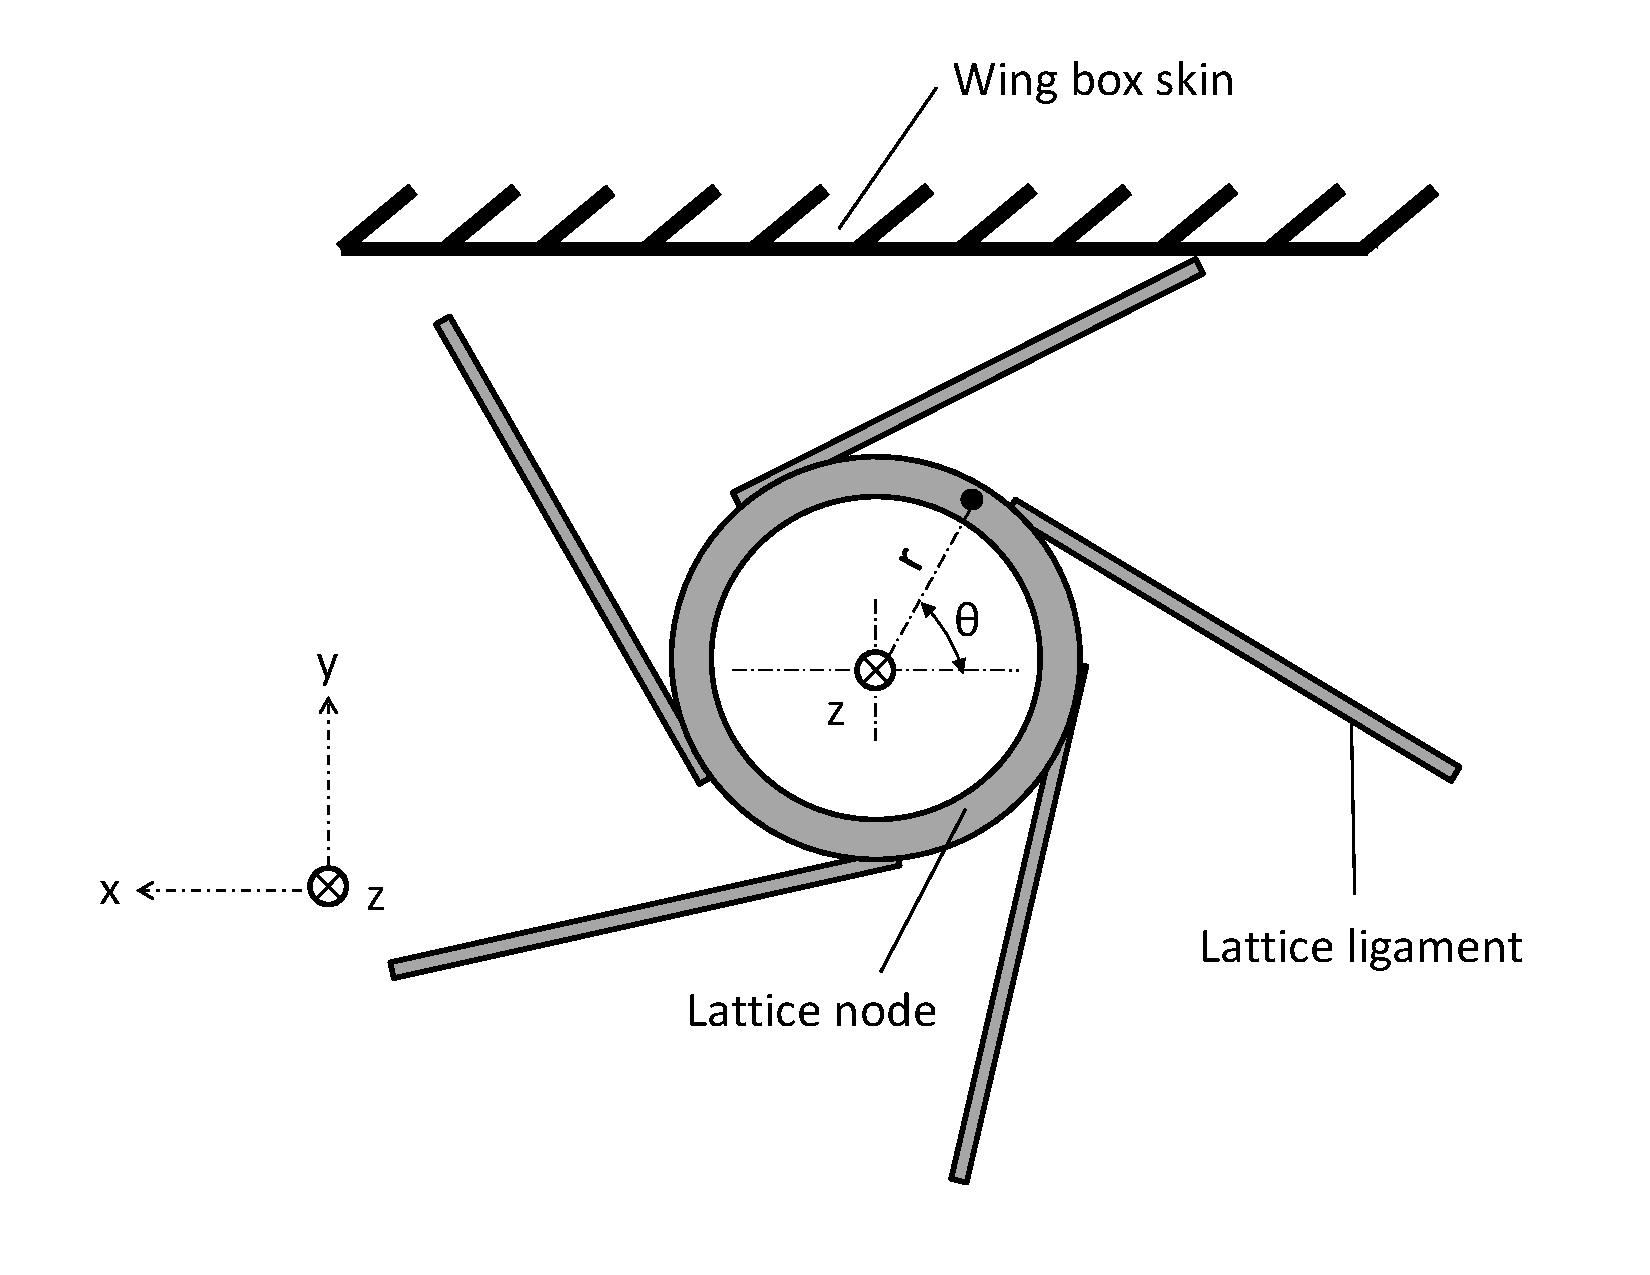
\includegraphics[width=0.6 \textwidth]{model/connection-SYS1}
  %     \caption[Local reference system at the lattice nodes]{Local reference system at the lattice nodes. The position of point in the lattice node faces will be determined by the radial distance $r$ to the origin, the angular position $\theta$ and the position $z$ along the node rotation axis.}\label{fig:connection-localSYS1}
  %   \end{figure}

  %   In the mentioned local reference system, a kinematic coupling constrain links the rigid body motion in $r$ and $z$ of a reference point located in the centre of the lattice node to those of a set of mesh nodes located on the lattice node faces. In the coupling definition, the reference point is the master node and the mesh nodes found in the faces of the lattice node are the slave nodes. This condition is visualized in Abaqus as shown in Figure \ref{fig:connection-localSYS2}.

  %   \begin{figure}[!htpb]
  %     \centering
  %     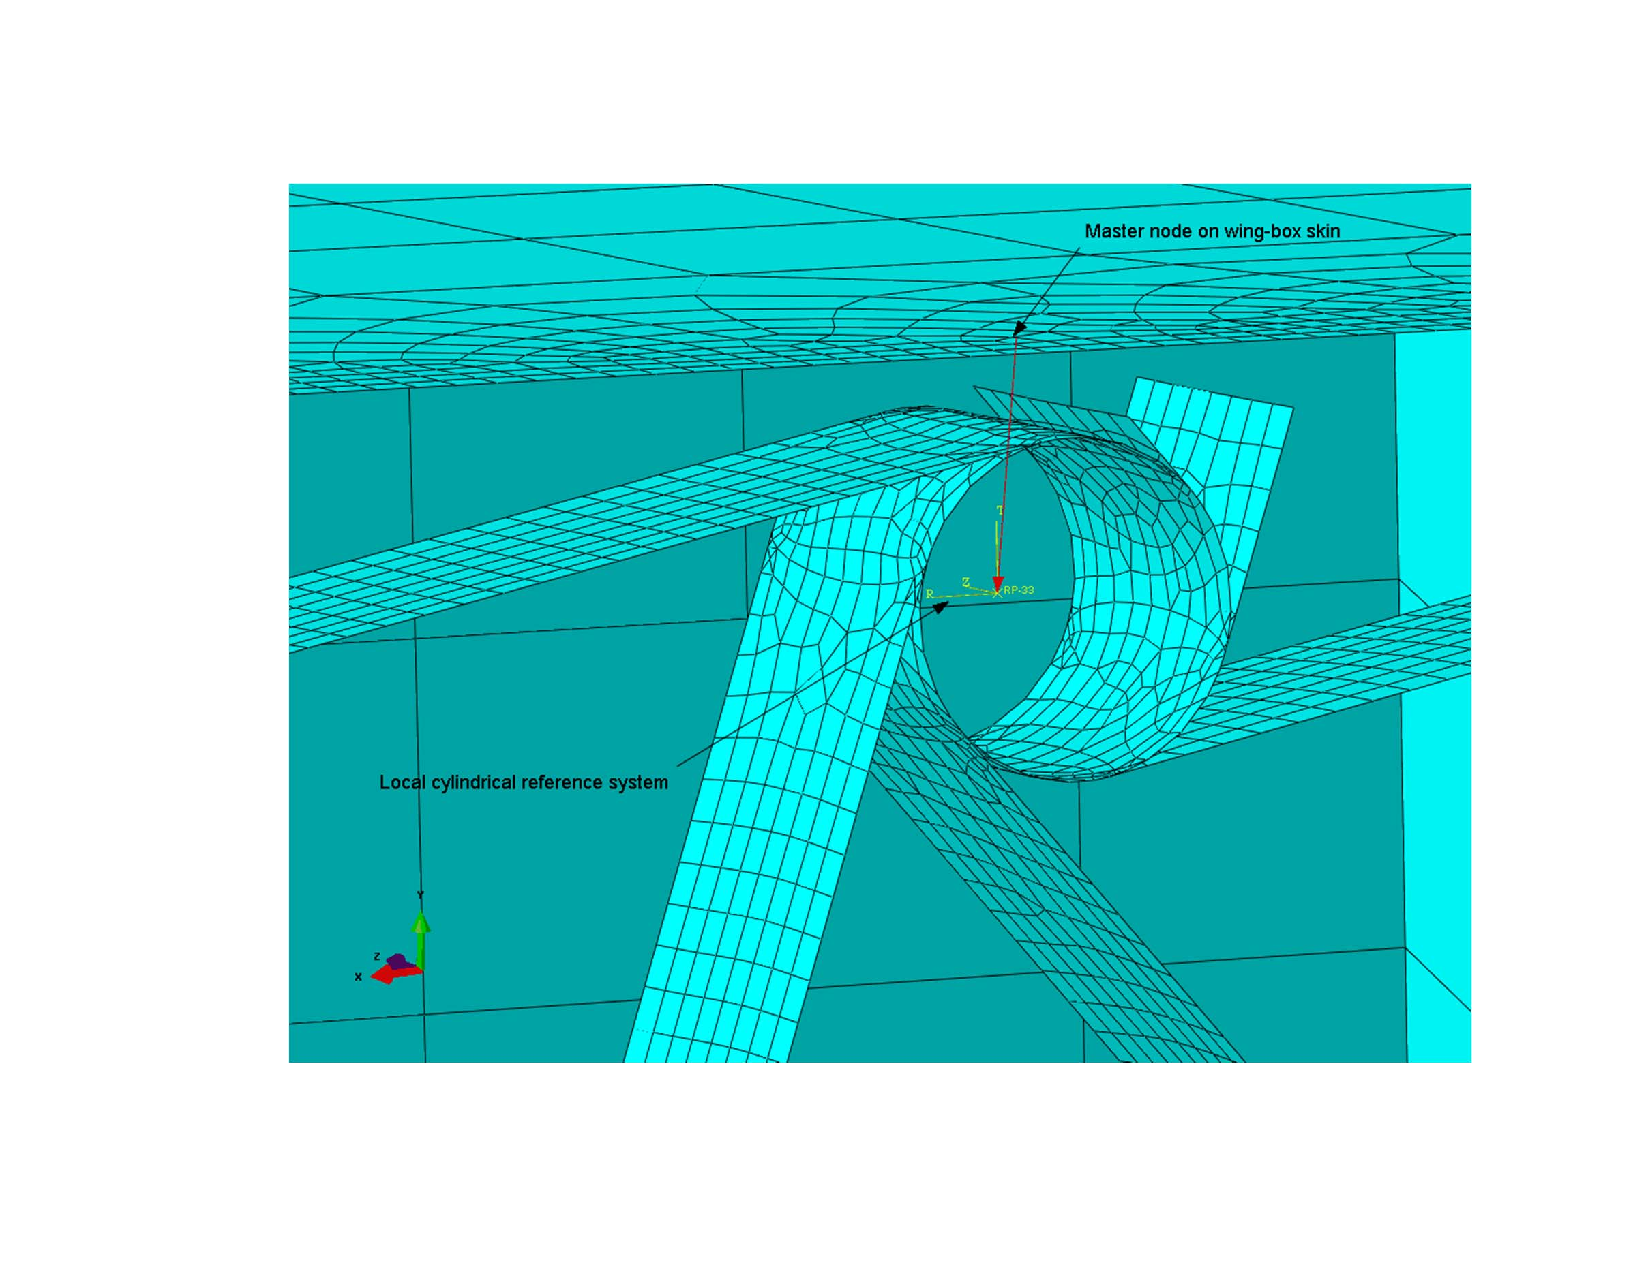
\includegraphics[width=0.7 \textwidth]{model/connection-SYS2}
  %     \caption[Coupling condition between the lattice node and the wing-box skin through a local reference system]{Coupling condition between the lattice node and the wing-box skin through a local reference system. }\label{fig:connection-localSYS2}
  %   \end{figure}

  %   Then, an additional coupling constrain is necessary to be establish in between the reference node that acts as the origin of the local cylindrical reference system and the wing-box skin. This is the same one that was previously establish when using a tyre part and shown in Figure \ref{fig:connection-tyre}. The only difference is that for this case the slave node is the reference point instead of a mesh node located in the center of the tyre.
